%%%%%%%%%%%%%%%%%%%%%%%%%%%%%%%%% Hauptteil %%%%%%%%%%%%%%%%%%%%%%%%%%%%%%%%%%

\chapter{Hauptteil}
\label{chap:Hauptteil}

\section{Projektdurchführung und Konzeption}

\subsection{Verwendete Hilfsmittel zur Durchführung des Projektes}
Das Projektseminar „Erstellung eines Zeitplan-Generators für Leichtathletikveranstaltungen“ wird von Thomas Baumer und Benedikt Bruckner, im Folgenden als die Studenten bezeichnet, unter Betreuung von Gerit Wagner durchgeführt. In der Anfangsphase des Projektes wird diskutiert, wie das Projekt umgesetzt werden soll und welche Software bzw. Programmiersprache zur Generierung des Zeitplans verwendet werden sollen.\\
Da der Zeitplan im HTML-Format erstellt werden soll, werden zum Erzeugen der Web-Dokumente sowie zur Verwendung von Web-Standards eine geeignete Programmiersprache und ein Editor benötigt. Zudem sind die Erstellung einer Desktop-App und eine ansprechende Oberflächengestaltung des Tools Ziele des Projektes. Darüber hinaus wird für eine optimale Zusammenarbeit im Team eine Möglichkeit gesucht, die ein paralleles Arbeiten an den Problemen ermöglicht. Auf welche Art und Weise diese Ziele erreicht werden sollen, wird im Folgenden detaillierter erläutert.\\
Für die Wahl einer Skriptsprache wird JavaScript verwendet. Vorteile dieser Lösung sind, dass für JavaScript eine Vielzahl an Dokumentationen, Bibliotheken und Tutorials existieren, so kann unter anderem bei der Programmierung auf die Bibliothek jQuery zurückgegriffen werden \cite{w3schools}.\protect{\footnote{\url{http://www.w3schools.com}
, zuletzt abgerufen am 30.11.16}} Ein weiterer Vorteil von JavaScript ist, dass eine einfachere Einbindung (z.B. durch eine öffentlich zugängliche Website) möglich ist. Die Verwendung von JavaScript ermöglicht die Erreichung aller gewünschten Ziele.\\
Als Editoren zur Erstellung von HTML- bzw. JavaScript-Code werden einerseits unter Windows Notepad++ und andererseits für Mac OS die Software Brackets verwendet, da diese Open Source-Editoren sind. Des Weiteren unterstützen diese Editoren viele Sprachen, u.a. JavaScript und HTML, die für die Entwicklung verwendet werden.\\
Für die Ausführung des Tools bzw. der verschiedenen HTML-Dokumente wird während der Entwicklung vordergründig der Browser Google Chrome verwendet, da dieser alle verwendeten Sprachen, Frameworks und Methoden unterstützt. Darüber hinaus werden auch die Browser Safari, Firefox und Opera für Tests miteinbezogen.\\
Für die Entwicklung einer Desktop-App wird die Software node.js in Verbindung mit dem Framework Electron eingesetzt. Dies bietet den Vorteil, dass für die Generierung des Zeitplans kein Browser benötigt wird. Deshalb ist es nicht notwendig, im JavaScript-Code für die jeweiligen Browser umständliche Anpassungen zu definieren. Ein weiteres Argument für die Erstellung einer Desktop-App mit der Software node.js in Verbindung mit dem Framework Electron ist, dass nach dem Erstellen des eigentlichen Programms mit dem Editor nur noch kleine Anpassungen vorgenommen werden müssen, um ein fertiges Programm zu erhalten. Ein eigenständiges Programm erleichtert die Bedienbarkeit bzw. die Nutzerfreundlichkeit, da der Nutzer die einzelnen HTML-Dokumente nicht abspeichern muss. Des Weiteren ermöglicht die tatsächlich entwickelte Desktop-App eine Nutzung des Zeitplan-Generators, wenn kein Internetzugang vorhanden ist. \\
Abgesehen von der Funktionalität soll das Zeitplan-Tool auch eine ansprechende Oberfläche besitzen, um die Benutzerfreundlichkeit zu erhöhen. Da der Zeitplan auch für große Leichtathletikveranstaltungen verwendet werden soll, ist die Oberflächengestaltung für die positive Wahrnehmung der Veranstaltung mitentscheidend. Um ein klares Design für den Zeitplan zu entwickeln, verwendet man das beliebte \ac{CSS}-Framework Bootstrap. Bootstrap bietet eine große Menge an Gestaltungsvorlagen für Oberflächengestaltungselemente, wie für Buttons oder Formulare. Diese ermöglichen eine einfache und schnelle Umsetzung eines ansprechenden Designs für das Zeitplan-Tool.
\protect{\footnote{\url{https://de.wikipedia.org/wiki/Bootstrap_(Framework)}
, zuletzt abgerufen am 30.11.16}} Der Entwickler benötigt also nur ein Basiswissen in HTML und CSS, um mit Bootstrap zu arbeiten. Dass Bootstrap mit allen gängigen Browsern kompatibel ist, ist ein weiterer Vorteil. Zudem wird eine angepasste Darstellung auf mobilen Endgeräten unterstützt.\protect{\footnote{\url{http://www.w3schools.com/bootstrap/bootstrap_get_started.asp}
, zuletzt abgerufen am 30.11.16}}\\
Des Weiteren wird die Verwendung einer Versionsverwaltungssoftware diskutiert. Eine Versionsverwaltung ermöglicht eine bessere Zusammenarbeit der Teammitglieder. Es werden beispielsweise das Wiederherstellen von alten Zuständen des Projekts und die Protokollierung ermöglicht, wodurch jede Änderung an den Dateien mit Autor und Datum nachvollzogen werden kann.  Zudem bietet eine Versionsverwaltung die Möglichkeit, Zugriffe und Entwicklungszweige zu koordinieren, was jedoch bei diesem Projekt aufgrund der Komplexität hinsichtlich der Projektteilnehmer nicht zwingend notwendig ist.\protect{\footnote{\url{https://git-scm.com/about} , abgerufen am 29.12.16}} Deshalb wird für die Durchführung des Projektes eine Versionsverwaltungssoftware genutzt.
Als Versionsverwaltungssoftware wird GitHub mit der \ac{GUI} des „GitHub Desktops“ verwendet, der eine einfache Zusammenarbeit auf dem Desktop ermöglicht.\protect{\footnote{\url{https://desktop.github.com} , zuletzt abgerufen am 14.01.17}}  \\
Nachdem alle für die Problemlösung benötigten Programme, Frameworks und Skriptsprachen festgelegt wurden, wird im Folgenden die Vorgehensweise zur Durchführung des Projektes beschrieben.

\subsection{Spezifikation des Rohtextes}

Ausgehend von den gemeinsamen konzeptionellen Überlegungen im Team wird zuerst der Rohtext spezifiziert, da dieser den Ausgangspunkt für die Entwicklung des Zeitplan-Generators darstellt. In diesem Prozess wird die genaue Form des Inputfiles festgehalten. Dabei ist es von besonderer Bedeutung, zu erkennen, an welchen Positionen die wesentlichen Veranstaltungsdaten wie das Datum, die Uhrzeit, die Kategorie und die Disziplin stehen.\\
Die erste Anforderung an den Rohtext ist, dass dieser das Dateiformat HTML besitzen soll. Dies ermöglicht eine genaue Navigation mit jQuery. Im Folgenden werden der Inhalt und die Struktur des Inputfiles näher spezifiziert, wobei zunächst der Aufbau eines Paragraphen (<p>-Tag) erläutert wird. Im listing ist beispielhaft der erste Paragraph in der zur Entwicklung verwendeten Ursprungsdatei aufgeführt. 
\lstset{language=html}
\lstinputlisting[caption=Beispiel eines Paragraphen, label=Ist:Beispiel eines Paragraphen]{listings/paragraphExample.html}
Im Testfile ergibt sich folgender Klartext (Tabelle 2.1), woraus eine verallgemeinerte Darstellung abgeleitet werden kann (Tabelle 2.2):\\
\begin{table}[h]
\caption{Beispielparagraph im Klartext}
\begin{tabular}{|l||l|}
\hline
Zeile 1: & „100m (Vorprogramm), Frauen + U20 + U18 – Zeitläufe“ \\
\hline
Zeile 2: & „Datum: 05.05.2016 Beginn: 12:00“ \\
\hline
\end{tabular}
\label{tab:Beispielparagraph im Klartext}
\end{table}
\begin{table}[h]
\caption{Verallgemeinerte Darstellung eines Paragraphen}
\begin{tabular}{|l||l|}
\hline
Zeile 1: & „Disziplin (Zusatzinformation), Kategorie(n) – Disziplin“ \\
\hline
Zeile 2: & „Datum Beginn“ \\
\hline
\end{tabular} 
\label{tab:Verallgemeinerte Darstellung eines Paragraphen}
\end{table}\\
Diese zwei Zeilen sind DOM-Elemente der Form <p class=“ev1“> ... </p>. Die relevanten Informationen werden mit Hilfe dieser Form identifiziert. \\
Die erste Zeile beinhaltet die Teilnehmerklasse(n) bzw. Kategorie(n) (hier: „Frauen + U20 + U18“) ungefähr in der Mitte der Zeile. Um die Teilnehmerklassen genau abzugrenzen, wird nach einleitenden bzw. beendenden Merkmalen der Teilnehmerklasse in der ersten Zeile gesucht. Die Teilnehmerklassen werden im Beispiel initiiert durch ein Komma und beendet durch einen Bindestrich. Dieses Muster ist für alle Paragraphen zutreffend, weshalb die Kategorie auf diese Weise in der ersten Zeile identifiziert werden kann. Des weiteren ist es möglich, dass mehrere Kategorien in einem Paragraphen enthalten sind. Dabei sind die Kategorien durch ein „+“ -Zeichen voneinander getrennt. 
In der Kategorie ist zudem die Information über das Geschlecht der Teilnehmer vorhanden. Mit Hilfe der Zeichenfolgen „weiblich“, „weibliche“ oder „Frauen“ bzw. „männlich“, „männliche“ oder „Männer“ kann dies festgestellt werden, da diese Schlüsselwörter das Geschlecht in allen Paragraphen eindeutig kennzeichnen. \\
Ein weiterer Bestandteil der ersten Zeile ist die Disziplin. Die Disziplin setzt sich aus den ersten Zeichen bis zur öffnenden Klammer und den letzten Zeichen nach dem Bindestrich zusammen.
Darüber hinaus kann der Inhalt der runden Klammern ebenfalls ein Teil der Disziplin sein. Ist eine der Zusatzinformationen „Hauptprogramm“, „Gala“, „Vorprogramm“ oder „Laufnacht“ der Inhalt der Klammern, ist die Zusatzinformation jedoch für die Bildung der Disziplin nicht relevant. Außerdem gibt es die Möglichkeit, dass keine runden Klammern mit Zusatzinformationen enthalten sind. Zusammenfassend ist die Zusatzinformation ein Teil der Disziplin, wenn eine Zusatzinformation im Paragraphen enthalten und diese nicht eines der ausgeschlossenen Wörter ist.
Im Beispiel entsteht die Disziplin „100m Zeitläufe“. Da das Vorprogramm eine irrelevante Zusatzinformation ist, wird sie bei der Bildung der Disziplin vernachlässigt.
\\
Die zweite Zeile enthält das Datum und die Uhrzeit. Der erste Eintrag in der zweiten Zeile ist „Datum“ gefolgt vom Datum selbst in der Form dd.mm.yyyy. Der zweite Eintrag in der zweiten Zeile ist „Beginn“ gefolgt von der Uhrzeit des Wettkampfstarts mit dem vierundzwanzig Studenformat hh:mm.\\
\\
Die für die Entwicklung verwendete Ursprungsdatei weist abgesehen von den enthaltenen Paragraphen folgenden Aufbau auf: In den ersten Zeilen des HTML-Dokuments steht die Überschrift (<title>Laufnacht und Sparkassen Gala 2016</title>) und ein JavaScript-Teil, der die Positionierung beim Laden des Files festlegt (script-Tag). Daraufhin folgen verschiedene Verweise, wie die Altersklassen in Form einer Tabelle (z.B. „Männer“ und „weibliche Jugend U20“ mit der Form <td class="tdMBar"><a ... /></td>) und alle Wettkampfbezeichnungen (z.B. <a ...>100m (Vorprogramm) - Zeitläufe<a/>), die von einem div-Tag umschlossen sind. 
Abgesehen davon kommt nach den Paragraphen in der verwendeten Ursprungsdatei immer eine Tabelle mit der Startnummer, dem Namen, dem Jahrgang, der Nationalität, dem Verein, der Saisonbestleistung und der persönlichen Bestleistung (<th>-Tag), sowie den verschiedenen Einträgen der Wettkampfteilnehmer (<td>-Tag). \\
Da jedoch nur die Paragraphen relevante Informationen für die Erstellung des Zeitplanes enthalten, wird dieser weitere Aufbau der Ursprungsdatei bei der Zeitplangenerierung vernachlässigt. 
Zusammenfassend muss das Inputfile im HTML-Format vorliegen und DOM-Elemente mit der Form <p class= „ev1“>...</p> enthalten, die als Inhalt die relevanten Daten haben. Der Rohtext kann grundsätzlich beliebigen HTML-Code beinhalten mit der Ausnahme des erläuterten Aufbaus eines Paragraphen, damit alle Daten im Anschluss richtig verarbeitet werden können.  

\subsection{Aufteilung der Entwicklungen in Pakete}

Dieser Unterpunkt gibt einen Überblick über die allgemeine Vorgehensweise zur Problemlösung, die später noch detaillierter erläutert wird. 
Zuerst wird festgelegt, dass das Problem den Zeitplan-Generator zu entwickeln in vier größere Teilprobleme bzw. Schritte unterteilt wird. Dies hat den Vorteil der Modularität der unterschiedlichen Funktionen. Die Implementierung der einzelnen Teilfunktionen ist leichter umzusetzen als die eines großen komplexen Problems. Zudem sind eine gute Testbarkeit der Funktionalitäten bzw. eine einfachere Wartung und besseres Debugging ermöglicht. Im Folgenden wird das Grundkonzept in den einzelnen Schritten für die Implementierung erläutert.\\
Der erste Schritt ist das Einlesen der Ursprungsdatei. Um mit dem Rohtext zu arbeiten, ist es notwendig, diesen zuerst zu identifizieren und einzulesen. Hier ist es die Aufgabe des Nutzers, die gewünschte Datei, die die zuvor spezifizierte Form aufweist, auszuwählen und einzulesen. Die Umsetzung dieser Funktionalität erfolgt im Web-Dokument FileUploader.\\ 
Der zweite Schritt ist, aus der Ursprungsdatei nur die relevanten Daten herauszufiltern. Hier werden praktisch nur noch alle relevanten Absätze betrachtet. Darüber hinaus bietet es sich an, die jeweiligen Paragraphen gleich nach erster und zweiter Zeile abzuspeichern (vgl. Abbildung 2.1). Dieses Teilproblem wird im HTML-File ParagraphHandler gelöst.
\begin{figure}[htbp]
  \centering
  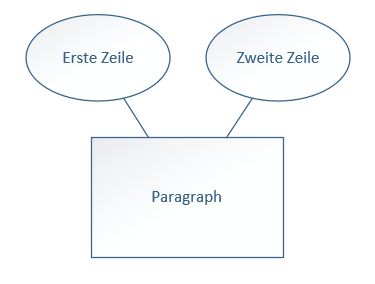
\includegraphics[width=0.4\textwidth]{Chen_StrucParagraph.png}
  \caption{Datenmodell eines strukturierten Paragraphen}
  \label{fig:Fig1}
\end{figure}\\
Anschließend werden diese Daten im dritten Schritt extrahiert, was im Web-Dokument Cleaner umgesetzt wird. Anhand bestimmter Suchkriterien werden das Datum bzw. die Uhrzeit in der zweiten Zeile und die Kategorie bzw. die Disziplin in der ersten Zeile von jedem Paragraphen erkannt und strukturiert abgespeichert. Hier ist es von Vorteil, dass ein Paragraph im ParagraphHandler unterteilt nach erster und zweiter Zeile abgespeichert wird. Um die Veranstaltungsdaten strukturiert ablegen zu können, wird der Datentyp Event (event) definiert (vgl. Abbildung 2.2).
\begin{figure}[htbp]
  \centering
  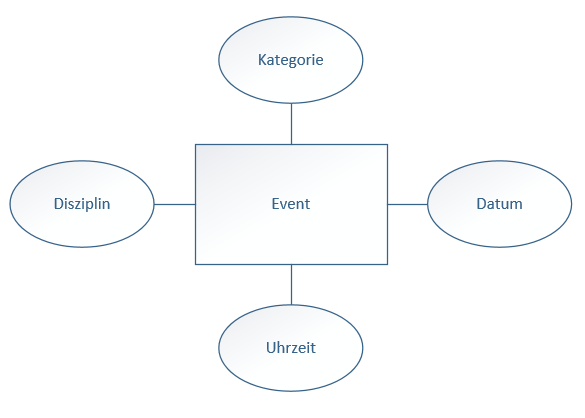
\includegraphics[width=0.6\textwidth]{Chen_Event.png}
  \caption{Datenmodell eines Events}
  \label{fig:Fig1}
\end{figure}\\
Im letzten Schritt wird schließlich im HTML-File GenerateTable der gewünschte Zeitplan aus den zuvor identifizierten Informationen dynamisch generiert. Für jeden Wettkampftag (eindeutiges Datum) wird dabei eine eigene Tabelle erzeugt, wobei als Überschrift für eine Tabelle das Datum dient. 
Eine Tabelle besteht aus einem Tabellenkopf (TableHead) und einem Tabellenkörper. Der Tabellenkopf ist die erste Zeile einer Tabelle. Der Eintrag in der ersten Zelle im Tabellenkopf ist stets das Wort Zeit. Die folgenden Inhalte der Zellen der ersten Zeile sind die jeweiligen Kategorien, die identifiziert wurden. Diese werden aszendierend und nach dem Geschlecht sortiert dargestellt. 
Der Tabellenkörper einer Tabelle kann aus mehreren Zeilen (TableRow) bestehen, wobei der jeweilige Beginn der Veranstaltung (Uhrzeit) in der ersten Spalte unter dem im Tabellenkopf definierten Titel Zeit angeordnet wird. Die Uhrzeit wird aufsteigend sortiert angezeigt. Jede Zeile beinhaltet Zellen (Cell), die gegebenenfalls die Disziplin oder keinen Inhalt (Content) als Eintrag haben. Darüber hinaus ist eine Zelle einer Kategorie aus dem Tabellenkopf zugeordnet. Die Disziplin wird also anhand des Datums, der Uhrzeit und der Kategorie zugeordnet (vgl. Abbildung 2.3).
\begin{figure}[htbp]
  \centering
  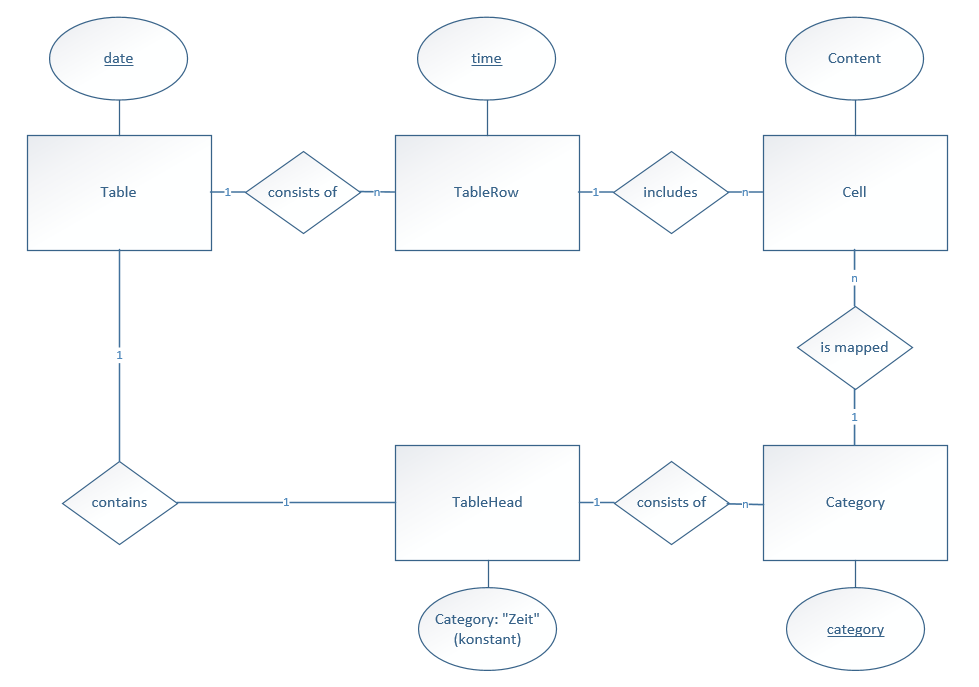
\includegraphics[width=0.8\textwidth]{Chen_Table.png}
  \caption{Datenmodell einer Tabelle}
  \label{fig:Fig1}
\end{figure} \\
Zusammenfassend werden also neben dem vorhandenen Inputfile vier HTML-Files mit JavaScript erstellt, die der Problemlösung dienen. Des Weiteren werden für die Desktop-App noch die Dateien index.html, main.js und package.json benötigt (vgl. Kapitel 2.2.6). Die genaue Vorgehensweise in den einzelnen Schritten wird im Folgenden genauer erläutert.

\section{Programmarchitektur und Ablauf}

\subsection{Allgemeine Festlegungen für die Web-Dokumente}

\subsubsection{Übersicht Programmablauf}
Wie in Punkt 2.1.3 beschrieben, werden zur Erstellung eines Zeitplan-Generators vier Web-Dokumente erzeugt. In diesem Unterpunkt wird der Programmablauf der Web-Dokumente als Übersicht dargestellt.
Die Web-Dokumente bauen aufeinander auf und haben die Ergebnisse der vorherigen HTML-Files als Vorbedingung. Im Folgenden werden die genaue Abfolge und die Ziele in den einzelnen Schritten erläutert.
\begin{figure}[htbp]
  \centering
  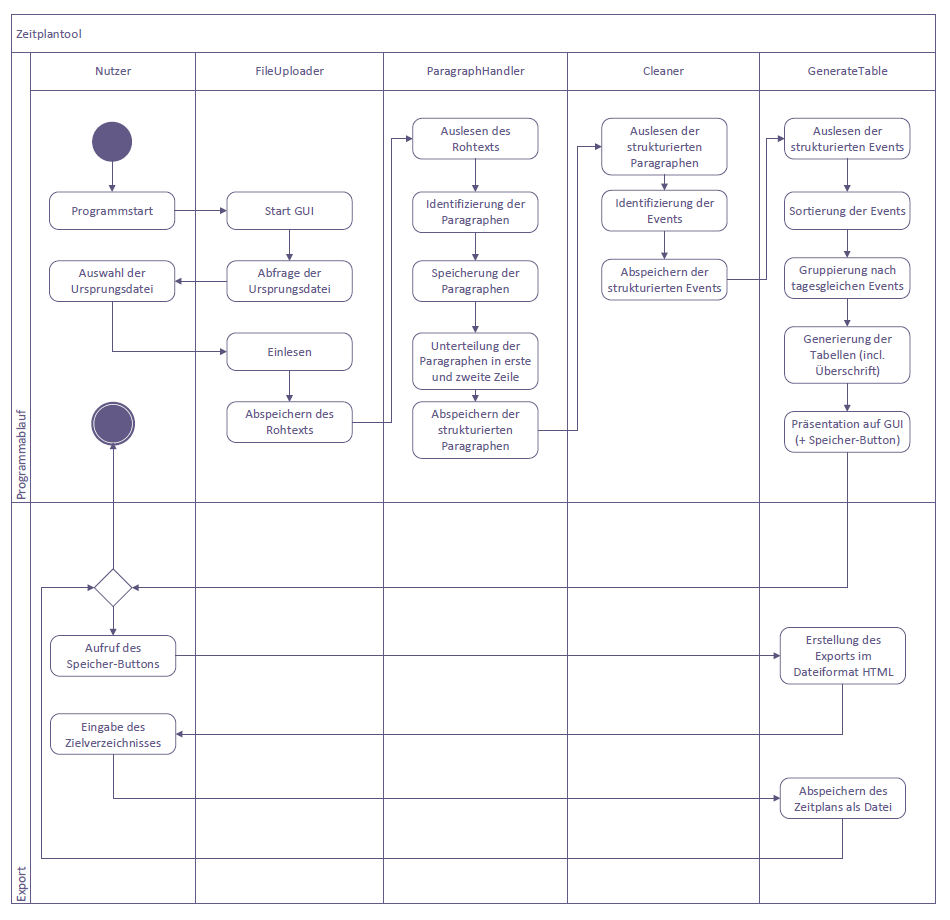
\includegraphics[width=1.0\textwidth]{GroberAblauf_UML.png}
  \caption{Übersicht Programmablauf}
  \label{fig:Fig1}
\end{figure} \\
\\
Der FileUploader ist der Ausgangspunkt bei der Erstellung des Zeitplans. Startet der Nutzer das Programm, wird die Nutzeroberfläche des FileUploaders angezeigt. Hier wählt der Nutzer das Inputfile, das in der spezifizierten Form vorliegen muss, aus. Dieses Inputfile wird eingelesen und im sessionStorage gespeichert. Anschließend leitet das Programm zum nächsten Schritt bei der Generierung einer Tabelle, dem ParagraphHandler, weiter.\\
Im ParagraphHandler ist es das Ziel, aus dem im sessionStorage gespeicherten Rohtext die Paragraphen, die für die Zeitplanerstellung benötigt werden, zu erhalten. Der Rohtext wird also zunächst aus dem sessionStorage ausgelesen. Danach werden die Paragraphen identifiziert und abgespeichert. Darüber hinaus ist es das Ziel, die Paragraphen gleich unterteilt nach erster und zweiter Zeile in einem Array abzuspeichern. Sind diese Ziele erreicht, wird zum HTML-Dokument Cleaner weitergeleitet.\\
Im Cleaner werden die Veranstaltungsdaten (Datum, Uhrzeit, Kategorie und Disziplin) als "events" extrahiert. Es werden zunächst die strukturierten Paragraphen ausgelesen und die events identifiziert. Anschließend werden die events als JSON im sessionStorage gespeichert. Somit werden die Veranstaltungen strukturiert, ähnlich zu einer Datenbank, abgelegt. Liegen die events im sessionStorage vor, wird zum HTML-Dokument GenerateTable weitergeleitet.\\
Im letzten zu erstellendem HTML-Dokument wird die Tabelle generiert. Dabei werden im ersten Schritt die strukturierten events ausgelesen. Um die Tabelle zu erzeugen, werden zunächst diese events sortiert und nach dem Datum gruppiert (tagesgleiche events). Anschließend wird der fertige Zeitplan auf der Nutzeroberfläche angezeigt und der Programmablauf ist beendet.\\
Darüber hinaus kann der Nutzer den erzeugten Zeitplan durch Aufruf des Speichern-Buttons exportieren. Im HTML-Dokument GenerateTable wird der Export im Dateiformat HTML erstellt. Hat der Nutzer das Zielverzeichnis angegeben, wird der Zeitplan als Datei abgespeichert.
 
\subsubsection{Weiterleitung zu den Web-Dokumenten}
Nachdem die Programmabfolge genauer erläutert wurde, wird nun die Weiterleitung zu den jeweiligen Web-Dokumenten erläutert. Die Web-Dokumente haben alle einen HTML-Kopf (HEAD) und einen HTML-Körper (BODY), die jeweils durch die gleichnamigen Tags eingeleitet und beendet werden. Im BODY wird standardmäßig die Weiterleitung zu den verschiedenen Dokumenten definiert. 
Die Weiterleitung zum jeweiligen Dokument erfolgt immer, wenn alle Ziele und Prozesse im vorherigen Schritt erreicht bzw. durchlaufen wurden (vgl. Kapitel 2.2.1.1). \\
Während der Entwicklungsphase wird jeweils ein Button implementiert, der beim Anklicken zu den verschiedenen Web-Dokumenten weiterleitet. Des Weiteren wird standardmäßig ein displayArea festgelegt, das die verschiedenen Ergebnisse der Web-Dokumente anzeigt. So ist ein einfaches Testen der Funktionalität und Debugging sicher gestellt. \\
Nach dem Abschluss der Programmierphase bzw. des Testens wird der Submit-Button und gegebenenfalls das displayArea im Code auskommentiert bzw. auf versteckt (hidden) gesetzt. Dies hat den Vorteil, dass man bei der Ausführung des kompletten Codes zur Erstellung der Tabelle durch das automatische Weiterleiten (Auto-Submit) zu den jeweiligen Web-Dokumenten Zeit spart. Zudem ist es für den Nutzer irrelevant, dass er beispielsweise das eingelesene File mit den unstrukturierten Daten angezeigt bekommt. Das displayArea wird nur bei den relevanten Seiten, die zur Benutzeroberfläche gehören, angezeigt. Es wird also nur die Aufforderung ein File einzulesen mit dem dazugehörigen Button und der erstellte Zeitplan mit dem Speichern-Button angezeigt. 
Bei Bedarf kann das Auskommentieren wieder rückgängig gemacht werden, was das Debugging bzw. die Erweiterung des Tools vereinfachen würde. 

\subsubsection{Festlegung des Titels und Einbindung von Bootstrap}
Im HEAD der Web-Dokumente wird immer der Titel festgelegt. 
Darüber hinaus erfolgt in den Dokumenten FileUploader und GenerateTable noch die Einbindung von Bootstrap im HEAD, da diese Web-Dokumente ein Teil der Benutzeroberfläche sind. 
Dabei werden für die Verwendung von Bootstrap immer drei Meta-Tags (<meta />) zu Beginn des HEADs deklariert. 
Dabei gibt das erste Meta-Tag den zu verwendenden Zeichensatz \ac{UTF-8} an. Die Verwendung von UTF-8 als Zeichensatz hat den Vorteil, dass alle Zeichen (auch Fremdwörter und Sonderzeichen) beliebig verwendet werden können.\protect{\footnote{\url{https://wiki.selfhtml.org/wiki/Zeichenkodierung}, aberufen am 23.11.16}} Des Weiteren ist UTF-8 von der \ac{IETF} und der \ac{ISO} als Norm definiert worden, was die Nutzung begünstigt.\protect{\footnote{\url{https://de.wikipedia.org/wiki/UTF-8}, abgerufen am 23.11.16}} \\
Das zweite Meta-Tag wird ebenfalls standardmäßig definiert, um eine bestmögliche Darstellung im Internet Explorer, auch in den älteren Versionen, zu gewährleisten.\protect{\footnote{\url{http://v4-alpha.getbootstrap.com/getting-started/browsers-devices/ }, aberufen am 02.12.16}}  Da der Internet Explorer jedoch nicht alle verwendeten Methoden bzw. Frameworks unterstützt, ist das Tool in diesem Browser nicht lauffähig. Für die Verwendung des Tools wird ein anderer Browser oder die Desktop-App benötigt.\\
Die Metainformation mit dem Namen viewport stellt sicher, dass die Website auch auf mobilen Geräten richtig dargestellt wird. Dies ist ein wichtiger Faktor, da heutzutage eine Vielzahl der Nutzer den mobilen Browser auf einem Smartphone verwenden und sich auf diesem Weg den Zeitplan anschauen. Durch den Ausdruck width=device-width wird eine genaue Anpassung der Website an die Bildschirmgröße des mobilen Endgeräts sicher gestellt. Des Weiteren wird die Möglichkeit des Zoomens nicht ausgeschlossen, da die Darstellung des Zeitplans auf einem mobilen Endgerät eventuell relativ klein ausfällt und der Nutzer die Informationen nur schwer erkennen kann. Das Zoom-Level wird beim ersten Laden der Website (initial-scale) mit dem Browser auf 1 gesetzt.\protect{\footnote{\url{http://www.w3schools.com/bootstrap/bootstrap_get_started.asp}, abgerufen am 02.12.16}} Darüber hinaus wird hier auch das für die Desktop-App verwendete Icon eingebunden.
Im Anschluss wird im HEAD die verwendete (minimierte) Bootstrap-CSS-Version definiert. 
Zudem werden in den Web-Dokumenten FileUploader und GenerateTable für die Verwendung von Bootstrap am Ende des BODYs noch die benötigten Skripte deklariert. Diese sind jQuery, das für Bootstrap JavaScript-Plugins benötigt wird, und das kompilierte JavaScript.\protect{\footnote{\url{http://holdirbootstrap.de/los-gehts/}, abgerufen am 02.12.16}} 

\subsubsection{Einbindung von jQuery}
Im ParagraphHandler wird das Framework jQuery eingebunden, dies ermöglicht ein einfaches Herausfiltern aller DOM-Elemente der Form eines Paragraphen (<p class=„ev1“>... </p>) aus der im sessionStorage abgespeicherten Ursprungsdatei. jQuery bietet unter anderem den Vorteil, dass es eine einfache und schnelle Möglichkeit bietet DOM-Elemente mit CSS-artigen Selektoren auszuwählen und zu bearbeiten. jQuery ermöglicht also DOM-Abfragen mit einer einfachen Syntax und bietet zudem Methoden, um wichtige Aufgaben mit sehr wenig Code zu erledigen \cite[S. 294ff.]{duckett}.\protect{\footnote{JavaScript \& jQuery - Interaktive Websites entwickeln, von Jon Duckett S.294ff}} Bei der Einbindung von jQuery in den Paragraph Handler gibt es drei verschiedene Möglichkeiten.\\
Eine Möglichkeit ist jQuery über Google zu laden. Dies hat den großen Vorteil, dass jQuery nicht extra geladen werden muss, wenn vorher Websites jQuery ebenfalls über die Google-API eingebunden haben. Dadurch wird die Performance bei der Ausführung des Codes verbessert. Muss jQuery trotzdem geladen werden, ist dies durch den Google-Server schnell möglich. \\
Eine weitere Lösung ist, dass man die aktuellste Version von jQuery.com nutzt. Hier kann einfach der Link der aktuellsten jQuery-Version als Quelle angegeben werden, was den Vorteil bietet, dass automatisch immer die neueste Version verwendet wird. \\
Die dritte Möglichkeit ist die Einbindung von jQuery über den lokalen Pfad, wo die Version nach dem Herunterladen abgespeichert wurde. Der Nutzer selbst muss jQuery nicht extra herunterladen, da jQuery in dem fertigen Paket des Zeitplan-Tools bereits enthalten ist. Der große Vorteil gegenüber den anderen Möglichkeiten ist, dass man keine Internetverbindung benötigt.\protect{\footnote{\url{http://www.html-seminar.de/jquery-tutorial.htm}, abgerufen am 27.11.16}} Der Nutzer kann den Zeitplan ohne Zugang zum Internet erstellen und lokal abspeichern. Ist der Nutzer beispielsweise gerade auf einer Leichtathletikveranstaltung und hat keinen Internetzugang, kann er trotzdem einen Zeitplan erstellen. Des Weiteren hat das lokale Einbinden den Vorteil, dass die Tabelle schneller als bei den anderen Möglichkeiten generiert wird, da durch die lokale Einbindung der Schritt des Herunterladens von jQuery wegfällt. Ein weiterer Vorteil ist, dass die Funktionaliät des Tools mit dieser Version getestet wurde. Das Programm ist also unabhänig von möglichen Änderungen in aktuelleren jQuery-Versionen und damit einhergehenden Problemen in der Kompatibilität. \\
Aufgrund dieser Argumente wird jQuery über den lokalen Pfad eingebunden.  
Darüber hinaus wird jQuery als Skript für Electron, Node.js und Bootstrap angegeben. 

\subsubsection{Allgemeine Definierungen im JavaScript-Code}
Im JavaScript-Code werden die restlichen Funktionalitäten der Web-Dokumente umgesetzt. JavaScript ist eine Skriptsprache, die HTML um Funktionalitäten erweitert und dynamische Informationen im Web realisiert. Das Skript wird in HTML-Dokumente mit dem script-Tag eingebettet. Dies ermöglicht beispielsweise, dass Benutzerinteraktionen ausgewertet bzw. Inhalte erzeugt oder verändert werden können. Diese Eigenschaften werden zur Erstellung eines Zeitplan-Generators benötigt. 
Standardmäßig werden im JavaScript-Code Methoden definiert, die das displayArea anzeigen und das Ergebnis des jeweiligen Web-Dokuments im sessionStorage abspeichern.

\subsection{Funktionalität des File-Uploaders}
  
\subsubsection{Festlegung des Designs des File-Uploaders}
Nachdem Bootstrap und der Titel im HEAD definiert wurden, wird im BODY die Gestaltung der Überschrift (Bootstrap Klasse "page-header") festgelegt. Die Überschrift wird separat, durch eine horizontale Linie unter der Überschrift, von den anderen Inhalten des File-Uploaders dargestellt. Dies wird mit dem div-Element in Verbindung mit der Klasse .page-header realisiert.\protect{\footnote{\url{http://www.w3schools.com/bootstrap/bootstrap_jumbotron_header.asp}, abgerufen am 02.12.16}} Die Überschrift gibt dem Nutzer den Hinweis, die Teilnehmerliste einzulesen.
Neben der Überschrift wird im File-Uploader noch ein Button plaziert, wo der User das gewünschte File auswählen kann. Da der Button einer der zentralen Bestandteile dieses Web-Dokuments ist, wird zuerst ein gesonderter grauer Bereich unterhalb der Trennlinie zur Überschrift definiert, wo später der Button plaziert werden soll. Dies wird mit der Bootstrap Wells-Klasse umgesetzt, die um ein Element einen grauen Bereich legt.\protect{\footnote{\url{http://www.w3schools.com/Bootstrap/bootstrap_wells.asp}, abgerufen am 02.12.16}} 
Für die Darstellung des Buttons selbst wird sich für ein Design entschieden, das an die verwendeten Farben der LG Telis Finanz-Website angelehnt sein soll (vgl. http://lg-telis-finanz.de). Dies unterstreicht eine konsistente Darstellung bei diesen Leichtathletikveranstaltungen. Bei den verschiedenen Button Styles von Bootstrap wird deshalb der Info-Button (.btn-info), der hellblau gefüllt ist und einen weißen Schriftzug hat, gewählt. Außerdem passt diese Darstellung mit dem vorher definierten grauen Bereich zusammen. Der Schriftzug des Buttons gibt dem Nutzer den Hinweis, die Datei hochzuladen. Außerdem enthält der Button noch die Funktion, auf einen Click zu reagieren. Die ausgelöste Methode clickedButton() wird im JavaScript-Teil definiert. Sie bewirkt, dass nach dem Click auf den Button der Click auf den Input (type: file) ausgeführt wird, der unsichtbar bzw. versteckt ist.
Außerdem wird im BODY noch der Input bestimmt, der vom Typ eines Files sein soll. Der Input wird am Anfang unter Verwendung von CSS ausgeblendet (style="display: none"). Dies ist eine saubere Lösung im Vergleich zu einschlägigen Vorschlägen aus dem Internet, wo der Fileinput mit einem Bild verdeckt wird (vgl. http://www.quirksmode.org/dom/inputfile.html).

\subsubsection{Einlesen und Abspeichern der Ursprungsdatei}
Im JavaScript-Code wird das Einlesen und Abspeichern der Ursprungsdatei umgesetzt. Dabei werden zuerst Variablen definiert, die die relevanten DOM-Elemente „fileInput“ und „displayArea“ abspeichern, um diese im JavaScript-Code verändern zu können bzw. um auf diese zugreifen zu können. 
Im Folgenden wird der User-Input als Event definiert. Dies ermöglicht, dass auf eine Dateiauswahl des Nutzers im Select-Auswahlmenü reagiert werden kann. Hat der Nutzer also eine Auswahl getroffen bzw. liegt eine Veränderung beim Inputfile vor (change), wird das Event ausgelöst. Bei der Auslösung des Events werden zunächst einige grundlegenden Dinge zur Ausführung des JavaScript-Codes festgelegt. 
Der Code arbeitet mit dem zuerst ausgewählten File (erste Stelle im Array) und prüft anschließend, ob das File den zuvor definierte Typ HTML aufweist. Wird an dieser Stelle erkannt, dass ein anderes Format vorliegt, wird das Event abgebrochen und es wird dem Nutzer eine Fehlermeldung („File not supported!“) im displayArea ausgegeben. 
Handelt es sich um ein HTML-File, ermöglicht die File Reader-\ac{API} das Auslesen des Textes. Hier wird zur Fehlervermeidung eine Verwendung eines falschen Texttyps vermieden. Um einen korrekten deutschen Text als Ergebnis zu erhalten, wird das File nach ISO-8859-1 enkodiert. Dies vermeidet beispielsweise, dass im Web-Dokument Umlaute nicht richtig dargestellt werden können. Sobald das File fertig geladen ist, wird der Inhalt des Eingangsfiles in der Variable „rawText“ gespeichert. Hier macht man sich die Methode onload bzw. das Attribut result der File Reader-API zunutze. Onload erkennt, wann das File komplett eingelesen wurde und result gibt den Inhalt des Files zurück.\protect{\footnote{\url{https://www.w3.org/TR/FileAPI/}, abgerufen am 24.11.16}} Darüber hinaus wird das Ergebnis des Einlesens, also die zuvor definierte Variable rawText, im sessionStorage abgespeichert. Die Datenspeicherung wird also an die aktuelle Browsersession gebunden, d.h. die Daten bleiben deshalb auch nur so lange gespeichert bis die Sitzung geschlossen wurde. Dies ermöglicht auch ein einfacheres Debuggen, da beispielsweise die fertige Tabelle selbst noch auf den Rohtext zugreifen könnte. Es ist also eine spätere Weiterverwendung der Zwischenergebnisse gewährleistet. Dies ist ein großer Vorteil gegenüber dem Versenden der Daten mit dem form-Tag. Zudem können andere Fenster im Browser die Daten während der Sitzung nutzen. 

\subsection{ParagraphHandler: Herausfiltern der Paragraphen aus dem Rohtext}

\subsubsection{Identifizierung und Speichern der relevanten Paragraphen}
Um mit der Ursprungsdatei arbeiten zu können, wird diese zunächst aus dem sessionStorage geladen. Dies geschieht in der Methode getRawText(). Anschließend wird der rawText im sessionStorage gespeichert, was in der Methode saveParagraphText(paragraphText) umgesetzt wird. Nach dem Speichern wird der Rohtext angezeigt, damit mit jQuery dieser durchlaufen und die Tags erkannt bzw. gefunden werden können. jQuery ermöglicht ein Finden aller Paragraphen mit der Klasse „ev1“, die in der Variable „\$html“ gespeichert werden. Mit dem Ausdruck „\$('p.ev1')“ werden nun alle Elemente mit dieser Eigenschaft zurückgegeben. Anschießend werden die Elemente in der jQuery-Auswahl mit der Methode clone() kopiert.\protect{\footnote{\url{http://www.w3schools.com/jquery/html_clone.asp}, abgerufen am 27.11.16}} Die Methode text() gibt nur den Textinhalt ohne Tags zurück. Nachdem die relevanten Informationen in der Variable \$html gespeichert wurden, kann der Inhalt der Seite bzw. der angezeigte Rohtext aus dem displayArea gelöscht werden. Dies wird durch das Setzen eines leeren Strings mit Hilfe der Eigenschaft innerHTML, die den Inhalt eines HTML-Elements speichert, realisiert.\protect{\footnote{\url{https://wiki.selfhtml.org/wiki/JavaScript/DOM/Element/innerHTML}, abgerufen am 27.11.16}} Anschließend ist es das Ziel, dass der Textinhalt der Paragraphen mit der Klasse ev1 der neue Inhalt der Seite sein soll. Dies wird mit der jQuery-Methode prepend(prepended text) ermöglicht, die den Inhalt (\$html) am Beginn der selektierten Elemente (pre) einfügt.\protect{\footnote{\url{http://www.w3schools.com/jquery/html_prepend.asp}, abgerufen am 27.11.16}} Da nun der Textinhalt der Paragraphen im displayArea angezeigt wird, kann der Inhalt nun mit der saveParagraphText(paragraphText)-Methode im sessionStorage abgespeichert werden.

\subsubsection{Vorbereitungen für ein strukturiertes Abspeichern der Paragraphen}
Im nächsten Schritt werden die Paragraphen noch strukturiert nach erster und zweiter Zeile als Array abgespeichert (vgl. Abbildung 2.1). Dies erleichtert das weitere Vorgehen bei der Generierung des Zeitplans. Dafür wird zunächst ein Konstruktor für einen strukturierten Paragraphen (StrucParagraph(firstLine, secondLine)) deklariert, wo die Paragraphen abgelegt werden können. Die Verwendung eines Konstruktors ermöglicht eine bessere und klare Verwendung im Code. Um ein Array aus Paragraph-Objekten (StrucParagraph) zu speichern, benötigt man zuerst den im sessionStorage gespeicherten unstrukturierten Textinhalt der Paragraphen. Mit dem Aufruf „sessionStorage.getItem('paragraphText')“ werden die Daten aus dem sessionStorage abgefragt und in der Variable „text“ gespeichert. Des weiteren wird das Array selbst definiert. Zudem werden drei Variablen deklariert, die die Anfangs-, Mittel- bzw. Endposition des Paragraphen wiederspiegeln. Diese Variablen helfen bei der Aufteilung des Textes in die zwei Zeilen. Bei der Initialisierung werden das Array und die Variablen zunächst auf leer bzw. 0 gesetzt. Darüber hinaus wird die Variable „patternTimeLength“ angelegt, die für die Zeichenlänge der Uhrzeit steht. Da sich die Uhrzeit immer aus zwei Stellen Stundenanzeige, einem Doppelpunkt und zwei Stellen Minutenanzeige zusammensetzt, ergibt sich in Summe eine Zeichenlänge von fünf. Deshalb wird die Variable bei der Initialiserung als Konstante auf fünf gesetzt.\\
Um den ganzen Text aus dem sessionStorage zu durchlaufen, benötigt man eine while-Schleife, die solange läuft, bis alle Daten erfasst und im Array abgespeichert wurden. Dabei wird die Schleife genau einmal für jeden Paragraphen durchlaufen. Es wird also zuerst ein Kriterium benötigt, um das Ende eines Paragraphen zu bestimmen. Da die Uhrzeit immer an letzter Stelle in den Paragraphen steht, wird die Position nach der Uhrzeit als Ende des aktuell betrachteten Paragraphen festgelegt. Nun wird nach einer Möglichkeit gesucht, um diese Stelle zu finden. Da die Startzeit immer fünf Zeichen hat und immer durch das Stichwort „Beginn:“ eingeleitet wird, könnte man nach dem Stichwort suchen und die restlichen Zeichen aufaddieren, um die gewünschte Position zu erhalten. Eine weitere Möglichkeit ist, dass man die Position der Uhrzeit mit Hilfe eines regulären Ausdrucks identifiziert. Dies hat den Vorteil, dass auch wirklich sichergestellt werden kann, dass eine valide Uhrzeit im Paragraphen gefunden wird. Der reguläre Ausdruck schreibt die Form vor, die die Uhrzeit aufweisen soll. Der gesamte reguläre Ausdruck setzt sich folgendermaßen zusammen:
\begin{verbatim}
([01]\d|2[0-3]):[0-5]\d
\end{verbatim}
Die Uhrzeit beginnt mit einer 0 oder 1 gefolgt von einer Zahl (0-9), im regulären Ausdruck als d für digit dargestellt, bzw. mit einer 2 gefolgt von den Zahlen 0, 1, 2, oder 3. Dies spiegelt die Stunden der Uhrzeit wieder. Nach den Stunden ist in der Uhrzeit der Doppelpunkt enthalten. Da die Minutenanzeige höchstens 59 anzeigen kann, erlaubt der reguläre Ausdruck an der ersten Stelle der Minutenanzeige nur eine Zahl zwischen 0 und 5. Die letzte Stelle der Uhrzeit darf eine Zahl zwischen 0 und 9 sein (digit). \\
Um im Paragraphen den Mittel- und Endpunkt zu finden und zu erhalten, wird die search- bzw. slice-Methode verwendet. Alternativ wäre hier auch die Verwendung von jQuery möglich gewesen. Die Methoden in Verbindung mit dem regulären Ausdruck werden aber verwendet, da die Paragraphen in der ersten und zweiten Zeile genug Regelmäßigkeit aufweisen, um diese Lösung zu benutzen. Die Methoden ermöglichen ein schnelles und einfaches Erhalten der gewünschten Positionen im Paragraphen.
Mit Hilfe der Methode search wird nun nach der im regulären Ausdruck definierten Form im Text gesucht und die Position der Übereinstimmung zurückgegeben.\protect{\footnote{\url{http://www.w3schools.com/jsref/jsref_search.asp}, abgerufen am 27.11.16}} Da die erste Stelle der Uhrzeit als Position geliefert wird, wird nun noch die patternTimeLength dazu addiert, um das Ende eines Paragraphen zu erhalten. Diese Position wird dann in der Variable endSliceP abgespeichert. Mit Hilfe dieser Variable kann also genau erkannt werden, wann der Paragraph endet. Der Paragraph wird nun mit Hilfe der slice-Methode aus dem ganzen Text abgeschnitten und in die Variable storageOneParagraph kopiert. Dabei braucht die slice-Methode als Parameterwerte einen Start- und Endpunkt, wobei der Endpunkt nicht mehr Teil des Ergebnisstrings ist.\protect{\footnote{\url{http://www.w3schools.com/jsref/jsref_slice_array.asp}, abgerufen am 27.11.16}} 

\subsubsection{Unterteilung der Paragraphen in erste und zweite Zeile}
Um die Paragraphen nun in die zwei Zeilen zu unterteilen wird nach einer Möglichkeit gesucht, um das Ende der ersten Zeile bzw. der Anfang der zweiten Zeile zu erkennen. Als Kriterium wird hier das Stichwort „Datum“ gewählt, da dies bei jedem Paragraphen am Anfang der zweiten Zeile enthalten ist und nicht Bestandteil der ersten Zeile ist. Um das Stichwort „Datum“ im Paragraphen zu finden, wird wieder die search-Methode, die die Position des Wortes zurückgibt, genutzt. Die Position wird in der Variable middleSliceLine (Mittelstück des Paragraphen) gespeichert. Für die Aufteilung des Paragraphen an dieser Stelle wird wieder die slice-Methode genutzt. Die erste Zeile geht von der Stelle 0 (Anfangsposition des Paragraphen bzw. startSliceP) des Paragraphen bis zur middleSliceLine-1. Hier wird eine Position noch abgezogen, um von der Stelle des Datums in die erste Zeile zu gelangen. Die zweite Zeile hat als Startpunkt die middleSliceLine und als Endpunkt die endSliceP. Die entstandenen Strings für die erste und zweite Zeile werden dabei gleich in den Variablen storageFirstLine bzw. storageSecondLine gespeichert. Im Anschluss werden nun noch die beiden Zeilen in einen StrucParagraph umgewandelt und diesem Array hinzugefügt. Dies wird mit der push-Methode umgesetzt. Im Array wird also der Paragraph in der Form, wie er angezeigt wurde, zwischengespeichert. Jetzt wird mit dem Aufruf text=text.slice(endSliceP) noch sichergestellt, dass der bereits abgearbeitete Paragraph aus dem Text weggeschnitten wird und im nächsten Durchlauf der darauffolgende Paragraph betrachtet wird.
Diese Anweisungen werden solange für jeden Paragraphen durchlaufen, bis alle Paragraphen mit der gewünschten Unterteilung in erster und zweiter Zeile zum Array hinzugefügt wurden.\\
\\
Im letzten Schritt werden die Paragraphen bzw. das Array noch gespeichert. Das Array wird als \ac{JSON} im sessionStorage abgespeichert, um Daten zwischen den HTML-Dokumenten austauschen zu können. JSON hat den Vorteil, dass das Format kompakter ist als HTML/XML.\protect{\footnote{JavaScript \& jQuery - Interaktive Websites entwickeln, von Jon Duckett S.374}} Zudem ermöglicht die Methode stringify(value) ein simples Parsen zu einem String. Das Array wird also als String in der Variable arrayJSON abgespeichert. 

\subsection{Cleaner: Strukturiertes Ablegen der Informationen aus den Paragraphen als Event}

\subsubsection{Vorbereitungen für die Identifizierung der Daten}
Nachdem die Paragraphen strukturiert nach der ersten und zweiten Zeile im sessionStorage abgelegt wurden, werden in diesem Schritt das Datum (date), die Uhrzeit (time), die Wettkampfbezeichnung (discipline) und die Wettkampfklasse (category) in den Paragraphen identifiziert und strukturiert als event abgelegt.\\
Dies wird im JavaScript-Code umgesetzt, der im Folgenden genauer erläutert wird. Um mit den Paragraphen zu arbeiten, wird zunächst das mit JSON im sessionStorage abgespeicherte Array (als String) wieder initialisiert. Dies wird mit der Methode getParagraphesText() realisiert, die die Paragraphen als String zurückgibt. Da für die Problemlösung das Paragraph-Objekt benötigt wird, wird der String wieder mit \ac{JSON} zu einem Array aus den Objekten „StrucParagraph“ geparst.\\
Im Anschluss werden für jedes StrucParagraph-Objekt die relevanten Daten identifiziert und abgespeichert. Da ein StrucParagraph-Objekt alle Daten für einen Wettkampf enthält, werden die Daten eines Paragraphen zusammengefasst als ein oder mehrere Events abgespeichert. Dies hat den Vorteil, dass die Daten korrekt und strukturiert abgelegt werden können. Die Definierung eines Events ermöglicht so später eine einfachere Erstellung der Tabelle. Der Datentyp Event wird also erzeugt. Er setzt sich aus dem Datum der Veranstaltung (date), dem Veranstaltungsbeginn (time), der Wettkampfklasse bzw. Kategorie (category) und der Wettkampfbezeichnung (discipline) zusammen (vgl. Abbildung 2.2). Dabei enthalten die Variablen alle relevanten Informationen zur Erstellung eines Zeitplans. Die Variablen sind vom Typ String. Um für die in einem Array gehaltenen StrucParagraph-Objekte jeweils ein Event zu erhalten, wird ebenfalls ein Event-Array definiert.\\
Um nun das Array aus StrucParagraph-Objekten zu durchlaufen, wird wieder eine for-Schleife benötigt. Dies ermöglicht, dass eine Reihe an Schritten für jeden einzelnen Paragraphen auf einmal umgesetzt werden kann. Die einzelnen Teilprobleme nicht auszulagern erscheint zwar unübersichtlich, aber diese Methodik erlaubt gleichzeitig, dass man im Verlauf die Daten in der Kopie (z.B. von der ersten Zeile) einfach verändern kann. 
Am Beginn der for-Schleife wird der Vorteil genutzt, dass im StrucParagraph-Objekt die erste und zweite Zeile eines Paragraphen getrennt abgespeichert wurden. Dies ermöglicht in diesem Schritt eine einfachere Identifizierung der Daten. Zuerst werden also Variablen definiert, die die erste und zweite Zeile des zu dem jeweiligen Zeitpunkt betrachteten Paragraphen wiederspiegeln. Anschließend werden die Daten, die in den jeweiligen Zeilen stehen, identifiziert.

\subsubsection{Identifizierung des Datums und der Uhrzeit}
Die erste und zweite Zeile können prinzipiell unabhängig voneinander bearbeitet werden. Im Code wird mit der Aufarbeitung der zweiten Zeile begonnen. Die zweite Zeile enthält am Anfang die Information des Datums der Veranstaltung und ungefähr ab der Mitte der Zeile steht der Veranstaltungsbeginn. Die Daten in der zweiten Zeile werden anhand von regulären Ausdrücken identifiziert. Dies ermöglicht, dass valide Informationen als Datum bzw. Veranstaltungsbeginn in der Zeile gefunden werden.\\
Der reguläre Ausdruck für das Datum setzt sich folgendermaßen zusammen:
\begin{verbatim}
(3[01]|[0-2]\d)\.(0\d|1[0-2])\.20\d\d
\end{verbatim}
Der reguläre Ausdruck setzt sich aus der Angabe des Tages, des Monats und des Jahres zusammen. Diese werden durch einen Punkt voneinander getrennt. Ein Tag beginnt mit einer 3 gefolgt von einer 0 oder einer 1. Die andere Möglichkeit ist, dass sich ein Tag mit einer 0, 1 oder 2 gefolgt von einer Zahl zwischen 0 und 9 (d für digit) zusammensetzt. Ein Monat besteht entweder aus einer 0 gefolgt von einem digit oder aus einer 1 gefolgt von einer 0, 1 oder 2. Somit sind alle Fälle vom ersten Monat Januar bis zum letzten Monat Dezember abgedeckt. Zum Schluss wird noch die Form des Jahres definiert. Die Jahreszahl beginnt mit einer 2 und einer 0 gefolgt von zwei Zahlen zwischen 0 und 9. 
In diesem regulären Ausdruck wird nur die Validität eines Datums und nicht die Korrektheit überprüft, da der reguläre Ausdruck nur zur Identifizierung eines Datums dient. D.h. Sonderfälle wie der Februar, der keine 3 an erster Stelle bei der Angabe des Tages haben kann, werden nicht auf Korrektheit geprüft.
Um den regulären Ausdruck zu finden, wird die Methode search verwendet, die die Anfangsposition des regulären Ausdrucks zurückgibt. Das Ergebnis wird in der Variable dateIndex gespeichert. Um auch die Endposition des Datums zu erhalten, wird die Variable patternDateLength mit dem Wert 10 definiert. Der Wert wird auf 10 gesetzt, da die Anzahl der Zeichen des Datums der Form (dd.mm.yyyy) in Summe immer 10 ergibt. Das Datum besteht also aus jeweils zwei Zeichen für die Angabe des Tages und des Monats, vier Zeichen für die Darstellung der Jahreszahl und zwei Punkten, um die Werte voneinander zu trennen. Mit Hilfe dieser Variablen wird nun das Datum in der zweiten Zeile erkannt. Mit der slice-Methode wird nun das komplette Datum zurückgegeben und in der Variable date gespeichert.\\
\\
Neben dem Datum wird noch die Uhrzeit in der zweiten Zeile identifiziert. Dies wird mit dem gleichen regulären Ausdruck umgesetzt, der bereits im Kapitel 2.2.3.2 genauer erläutert wurde. Durch die Kombination aus search- und slice-Methode wird wieder das gewünschte Ergebnis (hier: die Uhrzeit) geliefert. 

\subsubsection{Identifizierung der Disziplin}
Jetzt werden die Daten der ersten Zeile noch identifiziert. Zuerst wird die Disziplin identifiziert.
Da in der ersten Zeile in Klammern relevante oder irrelevante Zusatzinformationen für die Disziplin enthalten sein können, ist es nötig zuerst die relevanten Informationen zu erkennen. Zusatzinformationen sind die Begriffe „Gala“, „Laufnacht“, „Vorprogramm“ und „Hauptprogramm“. Sind diese Begriffe enthalten, braucht der Inhalt der Klammern nicht weiter betrachtet werden. Die Zusatzinformationen werden in dem Array cutOutOfBrackets abgespeichert. Um diesen Fall im Code abzubilden, wird zuerst eine if-Bedingung definiert. Diese wird nur durchlaufen, wenn Klammern enthalten sind. Sind Klammern vorhanden, wird mit Hilfe der split-Methode die Zeile in drei Teile zerlegt.\protect{\footnote{\url{http://www.w3schools.com/jsref/jsref_split.asp}, abgerufen am 04.12.16}} Der erste Teil (brokenFirstLineBrackets[0]) erstreckt sich vom Beginn der ersten Zeile bis zur öffnenden runden Klammer, der zweite Teil (brokenFirstLineBracketsHelper[0]) ist der Inhalt der runden Klammern und der dritte Teil (brokenFirstLineBracketsHelper[1]) ist der Text nach der schließenden runden Klammer. Nun wurde der Inhalt der Klammern isoliert und es kann überprüft werden, ob eine irrelevante Zusatzinformation enthalten ist. Dazu muss das Array cutOutOfBrackets durchlaufen werden. Ist eine irrelevante Zusatzinformation vorhanden, wird diese gelöscht. Falls eine relevante Zusatzinformation gefunden wird, wird diese zwischengespeichert. Nachdem die Fälle keiner und einer irrelevanten Zusatzinformation abgedeckt wurden, wird nun für die weitere Identifizierung die erste Zeile ohne Klammern und ohne den Inhalt der Klammern zusammengesetzt. Dies ist mit den zuvor definierten Variablen brokenFirstLineBrackets[0] und brokenFirstLineBracketsHelper[1] leicht umsetzbar.\\
Die Disziplin setzt sich aus mindestens einem Teil der ersten Zeile zusammen. Dabei ist der Teil vom Beginn der Zeile bis zum Komma (Klammern und Inhalt der Klammern sind nicht mehr vorhanden) immer ein Bestandteil der Disziplin. Der zweite Teil setzt sich gegebenenfalls aus dem Ende der ersten Zeile, dem Teil nach dem Bindestrich, zusammen. Darüber hinaus kann der Inhalt der Klammern, wenn dieser als relevant eingestuft wurde, ein Teil der Disziplin sein.
Zuerst speichert man die einzelnen Teile wieder in Variablen ab. Der erste Teil der ersten Zeile (bis zum Komma) wird in der Variable brokenFirstLineDiscipline[0] abgespeichert. Der mittlere Teil (brokenFirstLineDisciplineHelper[0]) erstreckt sich vom Komma bis zum Bindestrich und der dritte Teil (brokenFirstLineDisciplineHelper[1]) beginnt nach dem Bindestrich. Existiert der Klammerninhalt nicht oder wurde er als irrelevant eingestuft, kann die Disziplin aus dem ersten und gegebenenfalls dritten Teil bereits zusammengesetzt werden. Ist der Klammerninhalt relevant, wird dieser wieder in Klammern zwischen den beiden Teilen für die Bildung der Disziplin ergänzt. Das Ergebnis wird in der Variable discipline gespeichert.\\
\\
Nachdem die Disziplin erkannt wurde, werden gewisse Schlüsselwörter davon durch die allgemeingültigen Abkürzungen ersetzt. Dies hat den Vorteil, dass der Zeitplan bei der Erstellung kompakter und übersichtlicher wird. Die Wörter „Zeitläufe“, „Hindernis“, „Hürden“ und „Vorläufe“ werden dabei jeweils abgekürzt. Der Bezeichner „Finale“ wird ganz weggelassen, da im Fall keiner Angabe automatisch klar ist, dass es sich um ein Finale handelt. Für diese Konventionen dient der Zeitplan der Sparkassen Gala 2016 als Referenz. Prinzipiell ist hier eine ähnliche Lösung wie bei cutOutOfBrackets möglich bzw. die Funktionalität der Methode wäre als Replacement-Lösung abbildbar. Da aber bei cutOutOfBrackets nicht einmal ein Schlagwort gefunden werden muss, sondern nur Wörter verglichen und gegebenenfalls gelöscht bzw. ausgetauscht werden müssen, wird ein Array verwendet. Um die Wörter auszutauschen, wird der neue Datentyp Replacement erstellt, der das Schlüsselwort (key) und die passende Abkürzung (replacement) beinhaltet. Anschließend wird das Array replaceKeys definiert, wo die entsprechenden Replacement-Objekte aufgeführt sind. Dies hat den Vorteil, dass sofort erkannt wird, was abgekürzt werden soll und die Daten einfach gehalten werden. Des Weiteren ist es möglich schnell und einfach weitere abzukürzende Wörter in Zukunft hinzufügen. In der Methode wird die Ersetzung letztendlich durchgeführt. Als Parameterwert dient die zuvor jeweils festgestellte Disziplin eines StrucParagraph-Objekts. In der Methode wird das Array replaceKeys durchlaufen und bei einer Übereinstimmung des keys mit discipline wird diese durch die Abkürzung (value) ersetzt.

\subsubsection{Identifizierung der Kategorie}
Da die Disziplin erkannt und mögliche Abkürzungen eingeführt wurden, wird mit der Identifizierung der Kategorie fortgefahren. Die Kategorie setzt sich aus dem Geschlecht und der Altesklasse zusammen. Das Geschlecht wird benötigt, da ein Paragraph immer den Wettkampf für ein Geschlecht plus die verschiedenen Kategorien darstellt. Zuerst wird also festgestellt, ob es sich um einen Wettkampf für Frauen oder für Männer handelt. Um dies herauszufinden, wird die erste Zeile mit Hilfe der split-Methode in ein Array aller vorhandenen Wörter zerlegt. Dies ermöglicht, dass beim Durchlaufen das Array nach den Schlagwörtern „Frauen“, „weiblich“ und „weibliche“ durchsucht werden kann. Dazu wird der jeweils aktuelle Token (Leerraum wurde mit der trim-Methode entfernt) mit den Schlagwörtern verglichen. Diese Abfrage ermöglicht eine unkomplizierte Feststellung des Geschlechts. Wird eines dieser Schlagwörter gefunden, ist das Geschlecht weiblich („Frauen“). Ansonsten wird das Geschlecht auf männlich („Männer“) gesetzt. \\
Nun ist es notwendig die Altersklasse selbst noch zu identifizieren. Da in der ersten Zeile eines StrucParagraph-Objekts mehrere Kategorien enthalten sein können, muss die Variable, wo die Kategorien abgelegt werden sollen, ein Array sein. Für die Darstellung der Altersklassen werden die offiziellen Bezeichner des SC DHfK – Abteilung Leichtathletik (Stand 2016) verwendet. Es gibt Haupt-, Jugend- und ältere Altersklassen.\protect{\footnote{\url{https://www.leichtathletik-scdhfk.de/altersklassen/}, abgerufen am 04.12.16}} Der erste Schritt ist, dass das Vorkommen der Hauptklassen „Frauen“ und „Männer“ überprüft wird. Dazu wird das Array (brokenFLGender) wieder nach den verschiedenen Tokens durchsucht. Wird eine Hauptklasse gefunden, wird diese sofort durch den push-Befehl in das Array category mitaufgenommen.
Im Anschluss wird das Vorkommen von den Jugendklassen überprüft. Jugendklassen werden mit einem „M“ bzw. „W“ gefolgt von einem  „U“ und einer bzw. zwei Zahlen dargestellt. Da in der Ursprungsdatei aber diese Bezeichnung nicht zu finden ist, wird aus dem zuvor ermittelnden Geschlecht das Kurzzeichen erstellt. In der Ursprungsdatei werden die Jugendklassen immer durch ein „U“ gefolgt von einer bzw. zwei Zahlen eingeleitet. D.h. man vergleicht den ersten Buchstaben des gerade betrachteten Tokens mit dem „U“. Ist der erste Buchstabe ein „U“, wird das Kurzzeichen und der Token als Kategorie zum Array hinzugefügt. 
Die letzte Möglichkeit ist, dass eine ältere Altersklasse noch in der ersten Zeile vorhanden ist. Diese werden mit einem „W“ bzw. einem „M“ eingeleitet. Es wird also wie bei den Jugendklassen nur der erste Buchstabe des Tokens (W oder M) auf Übereinstimmung geprüft. Bei einem positivem Ergebnis wird die Kategorie dem Array hinzugefügt.\\
\\
Nachdem die Kategorie(n) erkannt wurde(n), wird aus dem Array category für jede Kategorie ein einzelnes Event (singleEvent) erstellt. Dabei sind die anderen Bestandteile des Events das Datum, der Veranstaltungsbeginn und die Disziplin. Diese werden wieder mit dem push-Befehl dem Array events hinzugefügt. Anschließend werden die events noch als JSON im sessionStorage gespeichert. 
Dieser Durchlauf wird für jeden Paragraphen wiederholt. Somit werden die Veranstaltungen strukturiert ähnlich zu einer Datenbank abgelegt.

\subsection{GenerateTable: Dynamische Erstellung des Zeitplans}

\subsubsection{Gestaltung des Speichern-Buttons}
Da die Tabelle dem Nutzer angezeigt wird und zusätzlich ein Speichern-Button integriert wird, wird für eine ansprechende und konsistente Darstellung wieder Bootstrap im Web-Dokument integriert. Im BODY wird nun der Speichern-Button, der dem Nutzer das lokale Speichern des Zeitplans ermöglicht, gestaltet. Diese Funktion ist für den Benutzer sehr sinnvoll, da es bei mehrmaligen Betrachten nicht notwendig ist die Website bzw. das Tool immer wieder aufzurufen. Der Speichern-Button wird für eine einheitliche Darstellung nach gleichen Design wie der „Datei auswählen“-Button beim FileUploader gestaltet. Der Button wird also wieder durch einen grauen Bereich vom restlichem Dokument abgehoben (Bootstrap Well-Klasse) und als Button-Style wird wieder auf den Info-Button zurückgegriffen (vgl. 2.2.2.1 Festlegung des Designs des File-Uploaders).\\
Wurde die Tabelle generiert, hat der Nutzer noch die Möglichkeit diese durch den Klick auf den Button lokal abzuspeichern. Es werden drei verschiedene Möglichkeiten für die Umsetzung des Speicherns diskutiert. Eine Möglichkeit ist, dass die Tabelle (<table>...</table>), die im sessionStorage gespeichert wurde, heruntergeladen wird. Eine weitere Lösung ist, dass das komplette HTML zum lokalen Speichern angeboten wird. Hier ist es dem Nutzer möglich das HTML-Dokument erneut runterzuladen. Die dritte Möglichkeit ist, dass das gesamte HTML-Dokument mit dem ausgeblendeten Button zum Abspeichern freigegeben wird. Dies hat den Vorteil, dass die lokale Kopie nur den eigentlichen Inhalt (die Tabelle) enthält. Zudem bleibt durch das Ausblenden die Funktionalität des Buttons erhalten. Ein mehrfaches Abspeichern ist bei dieser Lösung ebenfalls möglich. Aufgrund dieser Vorteile wird als Export das gesamte HTML-Dokument mit dem ausgeblendeten Button gewählt. 
Die Funktionaliät wird in der Methode createLocalCopy() umgesetzt. Da die dritte Möglichkeit umgesetzt wird, wird zuerst der Button ausgeblendet. Im Anschluss wird der komplette Seiteninhalt in der Variable text gespeichert. Darüber hinaus wird der Name der lokalen Kopie (Zeitplan.html) und der Typ des Dokuments (HTML) festgelegt. Anschließend wird ein neues File erstellt und es wird ermöglicht dieses lokal abzuspeichern.

\subsubsection{Sortierung der Events}
Im JavaScript-Code werden im ersten Schritt die als JSON im sessionStorage gespeicherten Events ausgelesen und in event-Objekte geparst. Im Anschluss werden die event-Objekte sortiert. Da für jeden Wettkampftag eine eigene Tabelle erzeugt wird, werden die Events zuerst nach dem Kriterium Datum sortiert. Die Sortierung zweiter Ordnung erfolgt nach der Zeit, da alle Wettkämpfe an einem Tag aufsteigend nach dem Beginn sortiert werden sollen. Darüber hinaus sollen die Events nach den Altersklassen geordnet im Zeitplan angezeigt werden. Es wird also noch nach der Kategorie sortiert. Die Sortierung nach diesen drei Kriterien wird in der ausgelagerten Methode sortEventsDateAndTimeAndCategoryOrder(events) vorgenommen.\\
Im ersten Schritt ist es nötig eine Möglichkeit zum Vergleichen der drei Kriterien mit den verschiedenen Werten eines Events zu finden. Durch die Umwandlung des Datums, der Uhrzeit bzw. der Kategorie zu einem Integer, ist es leicht möglich die entstehenden Werte miteinander zu vergleichen. Das Ziel ist es also aus den drei Kriterien einen Vergleichswert (Integer) der folgenden Form zu generieren: 
\begin{table}[h]
\caption{Vergleichswert zur Sortierung der Events}
\begin{tabular}{|l||c|c|c|c|c|c|}
\hline
 & Jahr & Monat & Tag & Stunden & Minuten & Kategorie \\
\hline
Beispiel & 2016 & 06 & 05 & 12 & 15 & 116 \\
\hline
\end{tabular}
\label{tab: Vergleichswert zur Sortierung der Events}
\end{table} \\
Anmerkung: Die Kategorie soll durch einen dreistelligen Integer dargestellt werden.\\
\\
Zuerst wird mit Hilfe der split-Methode das Datum und die Uhrzeit in ein Array aus Substrings aufgeteilt. Dabei werden für die Unterteilung der Punkt bzw. der Doppelpunkt verwendet. Nun ist es möglich das Datum und die Uhrzeit absteigend nach dem Jahr, dem Monat, dem Tag, den Stunden und den Minuten anzuordnen. 
Nach der Kategorie wird in der Methode getSortKeyTableHead(category) sortiert. Diese Funktion wird ausgelagert, da sie mehrmals benötigt wird. Die Kategorien sollen folgendermaßen geordnet sein: \\
weibliche Jugendklassen, Frauen, ältere Frauenklassen, männliche Jugendklassen, Männer und ältere Männerklassen. \\
Der Algorithmus gibt für die jeweilige Klasse einen dreistelligen Integer zurück, der die Altersklasse in das gewünschte Muster einordnet. Dabei werden für die jeweiligen Klassen bestimmte Basiswerte festgelegt. Für die Hauptklassen „Frauen“ und „Männer“ wird 200 bzw. 600 zurückgegeben. Diese Zahlen werden so festgelegt, damit für die Jugend- und älteren Klassen genug freie Werte zum Einordnen bleiben. Die weiblichen bzw. männlichen Jugendklassen werden initial mit dem Wert 100 bzw. 500 belegt. Dabei wird die jeweilige Zahl der Altersklasse zu 100 bzw. 500 addiert. Nach dem gleichen Prinzip wird auch bei den älteren Klassen ein Integer erstellt, wobei die Werte für die weiblichen Klassen bei 300 und für die männlichen Klassen bei 700 beginnen. Kann der Token keiner Kategorie zugeordnet werden und ist der Token nicht „Zeit“, wird der Wert an der rechten Seite der Tabelle hinzugefügt. Es wird der Integer 999 zurückgegeben.
Nun ist ein Integer entstanden, der ein Vergleichen der Events ermöglicht. Durch einfaches Subtrahieren von einem Integer erhält man einen Indikator zum Sortieren/Tauschen des Events. Die Methode sortEventsDateAndTimeAndCategoryOrder(events) gibt die sortierten Events zurück.

\subsubsection{Gruppierung nach tagesgleichen Events}
Nach dem Sortieren werden die Events auf die verschiedenen Tage aufgeteilt. Dies erfolgt in der Methode splitEvents(events). Es wird ein zweidimensionales Array initialisiert. In der ersten Dimension ist das Array nach dem Tag aufgeteilt und in der zweiten Dimension beinhaltet das Array ein weiteres Array aus den tagesgleichen Events. Die Variable indexReturnArray ist der Index der ersten Dimension, der angibt an welcher Stelle der aktuelle Tag ist. Die Variable currentDate definiert das Datum der aktuell betrachteten Gruppierung (das zu erstellende tagesgleiche event-Array). 
Nun wird für jedes Event aus dem übergebenen events-Array überprüft, ob es den selben Tag besitzt wie das zuletzt betrachtete Element. Dabei wird currentDate mit events[i].date verglichen. 
Wenn das Datum des zu erstellenden tagesgleichen Arrays (currentDate) mit dem des aktuell betrachtetem Event (events[i].date) übereinstimmt, wird das aktuell betrachtete Event ins returnArray in die zweite Dimension (an der Stelle indexReturnArray), wo die Events sind, gepusht.
Haben die Variablen einen unterschiedlichen Tag, wird die zweite Dimension um eine neue „Zeile“ erweitert. Der Zeiger indexReturnArray wird um eins erhöht und an dieser Stelle (neue Zeile bzw. den nächsten index im returnArray (ersteDimension)) wird ein neues Array initialisiert. Hier wird das aktuell betrachtete Event abgelegt und currentDate wird auf das neue Datum aktualisiert, sodass beim nächsten Vergleichen mit events[i].date wieder festgestellt werden kann, ob eine weitere Gruppierung benötigt wird.

\subsubsection{Generierung der Tabelle}
Im Folgenden wird die Tabelle und die Überschrift für jeden Tag (eventsSplitDays) erstellt, wobei für jeden Durchlauf der for-Schleife eine Überschrift und eine Tabelle erstellt wird. (vgl. Abbildung 2.3) Zuerst wird dem Seiteninhalt (pageContent) die Überschrift „Tagesprogramm für den“ und das aktuelle Datum der zugehörigen Events hinzugefügt (div-Tag). Dabei umgibt der graue Bereich wieder die Überschrift (Bootstrap Well-Klasse). 
Anschließend wird die Tabelle selbst noch generiert, was in der Methode generateTable(events) umgesetzt wird. Als Parameterwert bzw. Input müssen die sortierten und tagesgleichen Events vorliegen. \\
Das Ziel von generateTable(events) ist es als Output eine Tabelle (ohne Überschrift) mit dynamischen Inhalt und Tabellenkopf zu erzeugen. Die Zeilen und Spalten sind zusammen der Schlüssel für den Inhalt, wobei auch mehrere Events denselben Schlüssel haben können. Es können also auch zwei Events in einer Zelle stehen. 
Beim Aufruf generateTable(events) wird zunächst die Tabelle initialisiert. Die Tabelle wird wieder mit Bootstrap gestaltet. Dabei wird festgelegt, dass die Tabelle die Form der Bootstrap Hover Rows-Tabelle hat. Diese Klasse fügt beim Zeigen auf die jeweilige Reihe der Tabelle einen Hover-Effekt (graue Hervorhebung) hinzu.\protect{\footnote{\url{http://www.w3schools.com/bootstrap/bootstrap_tables.asp}, abgerufen am 08.12.16}}  Dieser Effekt unterstützt einerseits das Design und hilft andererseits dem Nutzer beim Finden der gewünschten Tabelleneinträge. \\
\\
Anschließend wird der Tabellenkopf generiert, den die Methode getTableHead(events) liefert. Als erstes wird ein Array (tableHead) definiert, das als Rückgabewert des Tabellenkopfs dient. Zum Array wird als erstes „Zeit“ hinzugefügt, da diese Spalte bei jedem Tabellenkopf gleich ist. Anschließend werden alle im event-Array vorkommenden Kategorien im Tabellenkopfs hinzugefügt, wobei jede Kategorie jeweils nur einmal im Tabellenkopf enthalten sein soll. Um die Kategorien dynamisch zum Array hinzuzufügen, wird für jedes Event geprüft, ob die Kategorie schon hinzugefügt wurde. Wenn eine neue Kategorie gefunden wird, wird diese dem Array hinzugefügt. Wenn alle Daten für den Tabellenkopf herausgefunden wurden, werden diese noch sortiert. Für die richtige Sortierung nutzt man wieder die Methode getSortKeyTableHead(token), die für die Vergleichbarkeit der Token einen Integer liefert. Anschließend kann durch das Ergebnis der Subtraktion zweier Integer (sortKeyA, sortKeyB) herausgefunden werden, ob die Werte getauscht werden müssen. Da bei der Akquirierung der Daten darauf geachtet wurde, dass die Werte eindeutig sind, können sie nicht übereinstimmen.
Wurden alle Werte richtig sortiert, wird das Array „tableHead“ zurückgegeben.
Nachdem die Daten für den Tabellenkopf ermittelt wurden, wird aus diesen Daten der HTML-Tabellenkopf erzeugt. Die Methode generateTableHead(tableHead) wandelt das Array tableHead zu einem HTML-String um, der der Tabelle hinzugefügt werden kann. Es wird festgelegt, dass der Tabellenkopf genau eine Zeile sein soll (tr-Tag). Anschließend wird das Array tableHead durchlaufen und es können die Tabellenkopfeinträge in den th-Tags eingefügt werden. Der Anfang und das Ende einer Zelle wird durch das th-Tag definiert. Wurden alle Einträge hinzugefügt, wird die für den Datensatz minimale und dynamische Tabellenkopfzeile zurückgegeben.\\
\\
Neben dem Tabellenkopf muss aus den Events noch der Tabellenkörper generiert werden. Zuerst werden die Objekte „Row(time, cells)“ und „Cell(category, content)“ definiert. Diese Objekte repräsentieren eine Zeile/Reihe (row) bzw. eine Zelle und werden für die Erstellung des Tabellenkörpers benötigt. 
Die Erstellung wird in der Methode generateTableBody(tableHead, events) umgesetzt. Zuerst werden aus den bereits nach dem Tag gruppierten Events diejenigen Events ermittelt, die zur selben Uhrzeit an dem jeweiligen Tag stattfinden. Diese Events müssen in die gleiche Zeile geschrieben werden. Die Methode getGroupedEvents(events) arbeitet nach dem gleichen Prinzip wie die Methode eventSplitDays(events). Der Unterschied ist, dass jetzt die Events mit dem gleichen Beginn und nicht mit dem gleichen Datum gruppiert werden. Es entsteht also ein Array, indem die verschiedenen Positionen die zeitgleichen Events wiederspiegeln.
Im Anschluss daran werden die zeitgleichen Events (groupedEvents) zu einer „TableRow“ (row-Objekt) geparst. Es wird ein Datenobjekt generiert, der einer Tabellenzeile ähnelt. Die Umwandlung der groupedEvents erfolgt in der Methode parseToRows(groupedEvents). Für alle zeitgleichen Events wird also eine Zeile erstellt, wobei ein Event in einer Zelle (Cell) steht. In einer Zelle wird die Kategorie und die Disziplin abgespeichert. Diese Zellen werden in einem Array (currentCells) zwischengespeichert. currentCells beinhaltet für eine Gruppierung von groupedEvents alle Kombinationen aus Kategorie und Disziplin, die aus den zeitgleichen Events herauszulesen sind. Da dadurch die Kategorien redundant sein können, muss das Array gekürzt werden. Kürzen bedeutet in diesem Fall, den Zelleninhalt der redundanten Kategorien zusammenzufügen.
Die Methode shortCells(cells) liefert die gekürzten Zellen als Array zurück. Es werden alle Zellen dem Array hinzugefügt, abgesehen von den Zellen, die dieselbe Kategorie besitzen. Als Primärschlüssel für dieses Zellen-Array wird also die Kategorie verwendet. Für diese Zellen wird der jeweilige Inhalt zusammengefügt, wobei zwischen den Inhalten ein Zeilenumbruch erfolgen soll. 
Nachdem die gekürzten Zellen vorliegen, kann eine Reihe aus dem Zellen-Array und der Uhrzeit erstellt werden. Dieser Vorgang wird für alle Tabellenzeilen wiederholt, wodurch das Array rows entsteht.
Zurück in der Methode generateTableBody(tableHead, events) wird nun als String der Tabellenkörper aus den rows erstellt. Dazu wird dem Ergebnis HTML-String immer die nächste Zeile aus rows, nachdem sie in getTableRow(row[i], tableHead) in das HTML-Format gebracht wurde, hinten angefügt.
Die Tabellenzeilen müssen als HTML-String dargestellt werden, was in der Methode getTableRow(row, tableHead) umgesetzt wird. Eine Zeile wird durch das tr-Tag initialisiert. Als erster Eintrag einer Reihe soll die Uhrzeit der gerade betrachteten Zeile stehen (td-Tag). Im Folgenden sollen die restlichen Zellen von links nach rechts anhand der aktuellen Kategorie erzeugt und gegebenenfalls befüllt werden. Für jede Spalte wird in der Reihe eine Zelle erstellt, egal ob diese Zelle als Inhalt eine Disziplin hat oder nicht (td-Tag). Mit der Methode getTableCellContent(cells, currentCategory) wird der Inhalt der gerade betrachteten Zelle geprüft, ob die betrachtete Zelle einen Inhalt hat. Wenn die Zeile eine Disziplin als Inhalt hat, wird diese zurückgegeben und zwischen den td-Tags eingefügt. Enthält die Zelle keinen Inhalt, wird ein leerer String zurückgegeben und zwischen den td-Tags eingefügt. Nach dem Aufruf dieser Methode, kann die Zelle durch das schließende td-Tag abgeschlossen werden. Wurde die komplette Reihe (row-Objekt) abgearbeitet, wird die Zeile durch das schließende tr-Tag beendet. \\
\\
Nachdem der Tabellenkopf und der Tabellenkörper generiert wurden, kann in der generateTable(events)-Methode die Tabelle beendet (</table>) und die komplette Tabelle zurückgegeben werden.
Der komplette Seiteninhalt wurde erstellt, wenn für alle tagesgleichen Events eine Tabelle erzeugt wurde. Ist das der Fall, wird die Tabelle im sessionStorage gespeichert und anschließend im displayArea angezeigt.

\subsection{Erstellung einer Desktop-App für den Zeitplan-Generator}

Um mit Electron eine Desktop-App zu erstellen, werden standardmäßig die Dateien index.html, main.js und package.json benötigt. Die index.html-Datei ist der Startpunkt für die Ausführung für den eigentlichen Inhalt des Fensters, main.js liefert die JavaScript-Logik und package.json hinterlegt alle wichtigen Eckdaten zu der App.\protect{\footnote{\url{http://t3n.de/news/electron-github-nodejs-chromium-656328/}, abgerufen am 20.12.16}} Für die Erstellung der Desktop-App wird das Quick-Start-Electron-Tutorial als Hilfestellung verwendet.\protect{\footnote{\url{http://electron.atom.io/docs/tutorial/quick-start/}, abgerufen am 20.12.16}}  Im Folgenden werden die drei benötigten Dateien näher erläutert.\\
\\
In dem Dokument index.html wird der Inhalt der Website, der angezeigt werden soll, festgelegt.
Im HEAD werden standardmäßig der zu verwendenden Zeichensatze UTF-8 und der Titel deklariert. Zudem wird ein Icon für index.html definiert. Ein eigenes Icon ist bei vielen Desktop-Apps ein Standard, weshalb für den Zeitplan-Generator auch ein eigenes Icon gestaltet wird. Zudem erscheint das Tool mit einem Icon benutzerfreundlicher. Das Icon wird mit der Software Iconion erstellt, die eine Vielzahl an Symbolen, Styles und Einstellungsmöglichkeiten zur Icon-Gestaltung frei zur Verfügung stellt.\protect{\footnote{\url{http://iconion.com/de/}, abgerufen am 20.12.16}}  Das Icon wird ähnlich wie Teile der Oberfläche der Web-Dokumente FileUploader und GenerateTable wieder hellblau gestaltet. Zudem ist ein Dokumentensymbol in weißer Farbe Bestandteil des Icons, das den Zeitplan wiederspiegeln soll (vgl. Abbildung 2.5).
\begin{figure}[htbp]
  \centering
  
\includegraphics[width=0.2\textwidth]{Icon.png}
  \caption{Icon der Desktop-App}
  \label{fig:Fig1}
\end{figure}\\
Da das Web-Dokument FileUploader.html der Ausgangspunkt des Zeitplan-Generators ist, wird im JavaScript-Code eine Weiterleitung deklariert, die automatisch zu den vorherig beschriebenen Web-Dokumenten mit dem Programmablauf weiterleitet. index.html wird verwendet, weil es ein Standard ist auf diese Weise eine Website zu starten. 
In der Datei package.json werden wichtige Informationen zum Packen bzw. Erstellen der einzelnen HTML-Files zu einer eigenständigen App hinterlegt. Es werden standardmäßig der Name, der Produktname, die Version, das main-Feld, die Abhängigkeiten (dependencies) und drei Skripte definiert. Das main-Feld gibt das Script, welches den Hauptprozess (main.js) auslöst, an. Unter Abhängigkeiten versteht man die Angabe der benötigten Versionen von jQuery, electron und des electron-packagers. Die Skripte sind eine Vordefinierung für die Befehle der Kommandozeile, um die Desktop-App zu packen. Dadurch muss der Nutzer den Befehl für den electron-packager nicht selbst schreiben, sondern kann eine Abkürzung über das Skript nehmen. Die Skripte werden für die Betriebssysteme Mac OS, Windows und Linux definiert. Durch Electron und das Packen des electron-packagers wird die Ausführbarkeit der Desktop-App auf diesen Betriebssystemen gewährleistet. Dies ist ein großer Vorteil, da nicht für jede Umgebung eine eigene App programmiert bzw. viele Anpassungen vorgenommen werden müssen. Für das Packen der Desktop-App ist es zuerst nötig Node.js, Electron und den electron-packager zu installieren. Anschließend wird in der Kommandozeile durch den Aufruf der jeweiligen Befehle für die Skripte im Verzeichnis der App diese selbst installiert. Die Befehle für die jeweiligen Betriebssysteme sind:
\lstset{language=html}
\lstinputlisting[caption=Anleitung für die Installation des Tools, label=Ist:Anleitung für die Installation des Tools]{listings/Tool_Anleitung}
Die dritte Datei main.js liefert die JavsScript-Logik für die Desktop-App selbst. Dies beinhaltet das Erzeugen von Fenstern und das Handeln von System-Events. Zuerst werden eine Referenz für ein Fenster-Objekt und das Icon definiert. Die Größe des Browserfensters, wo die HTML-Dokumente ausgeführt werden, wird festgelegt. Zudem wird der Content der Desktop-App, index.html, geladen. Anschließend wird definiert, wann die Browserfenster erzeugt bzw. beendet werden. Das Browserfenster wird erzeugt, sobald Electron die Initialisierung abgschlossen hat. Die App wird beendet, wenn alle Browserfenster geschlossen wurden. Hier wird noch eine Ausnahme für Mac OS definiert, da hier die Programme standardmäßig erst durch das Kommando Cmd+Q geschlossen werden. Wird in der App-Version für Mac OS wieder auf das Icon geklickt, wenn die App nicht geschlossen ist, wird das Fenster der App wieder erzeugt.

\section{Evaluierung des Projektverlaufs}
\subsection{Projektbeginn und Konzeption}
Das Projekt Erstellung eines Zeitplan-Generators für Leichtathletikveranstaltungen wurde Mitte Oktober 2016 gestartet. Zuerst wurde das Problem einen automatischen Zeitplan aus einer Ursprungsdatei zu erzeugen definiert. Darüber hinaus wurden die zu erreichenden Ziele bestimmt. Es wurde festgelegt, dass der Zeitplan vollständig, richtig, konsistent und dynamisch generiert werden soll. Zudem ist der Zeitplan in Anlehnung an die Referenztabelle der Sparkassen-Gala 2016 und im HTML-Format zu erstellen.\\
Nach der Eingrenzung der Problemstellung und erster Zieldefinierungen wurde mit der Konzeption begonnen. Das Problem wurde in mehrere Pakete aufgeteilt und es wurden die benötigten Hilfsmittel für die Umsetzung festgelegt. Zudem wurde die für die Entwicklung verwendete Ursprungsdatei analysiert und ein erstes, eher provisiorisches Datenmodell erstellt.
Diese Phase wurde schnell bearbeitet, um mit dem aufwändigsten Schritt der Implementierung beginnen zu können. Dabei war es ein großer Vorteil, dass das Projektteam nur aus zwei Personen besteht. Es wurde durch die enge Zusammenarbeit stets schnell eine für alle zufriedenstellende Lösung für auftretende Probleme bzw. Konzeptionsentscheidungen gefunden.\\
Außerdem wurde sich auf die Umsetzung der agilen Werte der Softwareentwicklung geeinigt. Dies bedeutet, dass im Projekt schnell auf Veränderungen reagiert wird und gewünschte bzw. erwartete Ziele des Nutzers umgesetzt werden. Menschen und Interaktionen bzw. die Zusammenarbeit mit dem Nutzer stehen im Vodergrund. Zudem steht bei dieser Vorgehensweise die Funktionalität über einer umfassenden Dokumentation am Code.\protect{\footnote{\url{https://de.wikipedia.org/wiki/Agile_Softwareentwicklung\#Agile\_Werte}, abgerufen am 03.01.17}} Verwendete Techniken waren unter anderem das evolutionäre Prototyping sowie das Spiralmodell.
\begin{figure}[htbp]
  \centering
  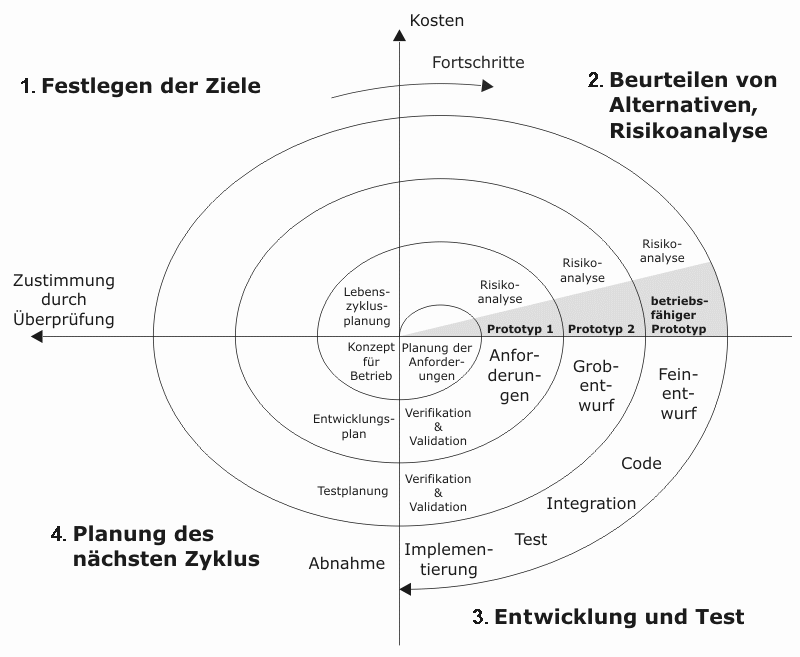
\includegraphics[width=0.7\textwidth]{Spiralmodel_nach_Boehm.png}
  \caption{Spiralmodel nach Boehm}
  \label{fig:Fig1}
\end{figure}\\
Während der Entwicklung wurden stets neue Ziele definiert und verschiedene Alternativen diskutiert. Zudem wurde das aktuelle Programm und die gefundenen Lösungen Tests unterzogen und die Projektfortsetzung geplant.\protect{\footnote{\url{https://de.wikipedia.org/wiki/Spiralmodell}, abgerufen am 03.01.17}} Dabei wurde das Programm schrittweise nach den gewünschten und vom Auftraggeber erwarteten Funktionalitäten erweitert. Das übergeordnete Ziel ist es ein Programm mit den Grundfunktionalitäten zu erhalten.\protect{\footnote{\url{https://de.wikipedia.org/wiki/Prototyping_(Softwareentwicklung)\#Evolution.C3.A4res\_Prototyping}, abgerufen am 03.01.17}} Die verschiedenen Prototyp-Versionen und die Abstimmungen bei der Implementierung werden im Folgenden genauer erläutert.

\subsection{Erste Implementierungsphase und Problemabstimmung}
Nachdem erste konzeptionelle Entscheidungen getroffen wurden, wurde mit der Implementierung des Zeitplan-Generators begonnen. Dabei wurde aufgrund der guten konzeptionellen Vorarbeit sehr schnell eine vorläufige Lösung des Problems erzeugt.\\
Im Anschluss an die erste Implementierungsphase wurden einige Probleme bei der Implementierung abgestimmt. Zuerst wurde die Aufteilung des Problems in vier Pakete hinterfragt. Da jedoch genau vier Teilprobleme identifiziert werden konnten, wurde diese Möglichkeit der Lösung beibehalten. Zudem hat dies den Vorteil der Modularität.\\
Des Weiteren stellte sich die Frage, ob eine automatischer Weiterleitung zu den jeweiligen Web-Dokumenten integriert werden soll. Diese Möglichkeit wurde anstatt der Weiterleitung durch einen Klick auf die verschiedenen Buttons in den jeweiligen Web-Dokumenten umgesetzt. Dies hat den Vorteil der schnelleren Zeitplan-Generierung. Des Weiteren ist eine automatische Weiterleitung sinnvoll, da für den Nutzer die Zwischenschritte bei der Erstellung des Zeitplans nicht relevant sind. \\
Ein weiterer Diskussionspunkt war, ob die Ursprungsdatei automatisch ausgewählt und eingelesen werden soll. Dies wurde aufgrund der Möglichkeit mehrerer möglicher Teilnehmerlisten, die der Nutzer zu unterschiedlichen Zeitpunkten einlesen möchte aber nicht verwirklicht. Es wurde also an der aktuellen Lösung, dass der Nutzer die Ursprungsdatei einliest, festgehalten.\\
Die Art der Erkennung der Uhrzeit und des Datums wurde ebenfalls diskutiert. In der ersten Implementierungsphase werden diese anhand der Regelmäßigkeit der Zeichenposition in der zweiten Zeile eines Paragraphen identifiziert. Betreuer Gerit Wagner riet hier die Verwendung von regulären Ausdrücken. Diese ermöglichen, dass valide Werte der Uhrzeit bzw. des Datums identifiziert werden können.\\
Ein Problem in der ersten Implementierungsphase ist, wie mit der Information in den teilweise vorhandenen Klammern in den Paragraphen umgegangen werden soll. Es wurde festgelegt, dass es nicht relevante und relevante Zusatzinformationen in den Klammern gibt. Dabei wurden die Wörter „Gala“, „Vorprogramm“, „Hauptprogramm“ und „Laufnacht“ als irrelevante Zusatzinformationen eingestuft. Die relevanten Informationen hingegen sollen Teil der Disziplin sein.\\
Die Identifizierung der Art der Veranstaltungen (Geschlecht) mit den Tokens „weiblich“, „weibliche“ und „Frauen“ wurde ebenfalls angesprochen. Es stellte sich heraus, dass auf diese Weise eine eindeutige Zuweisung möglich ist. Diese Art der Ermittlung ist also ausreichend und kann beibehalten werden.\\
Darüber hinaus wurden die verschiedenen Kategorien bzw. Altersklassen diskutiert. In der ersten Implementierungsphase wurde als Übergangslösung das maximale Alter auf dreißig Jahre gesetzt, wenn kein Alter ermittelt werden konnte. Des Weiteren wird für jedes erlaubte Alter in aufzählender Weise eine eigene Spalte für Männer als auch für Frauen erstellt. Es wurde das neue Ziel definiert, dass allgemeine Bezeichner der Leichtathletik-Altersklassen verwendet werden sollen. Zudem wurde die Zusammenfassung der Kategorien bei gleichen Disziplinen diskutiert. Aufgrund der besseren Übersichtlichkeit und Konsistenz der Daten wurde festgelegt, dass für jede Kategorie eine Spalte im Zeitplan erstellt werden soll. Um den Zeitplan trotzdem möglichst kompakt darzustellen, wurden allgemeingültige Abkürzungen eingeführt bzw. der Bezeichner „Finale“ weggelassen. \\
Ein weiteres Problem ist, dass eine Lösung für zeitgleiche Veranstaltungen für eine Altersklasse gefunden werden muss. Es wurde festgelegt, dass diese Veranstaltungen in einer Zelle stehen und durch einen Zeilenumbruch voneinander getrennt werden. Um eine bessere und effizientere Datenhaltung zu gewährleisten, wird das Array category im event aufgelöst, sodass für jeden category-Eintrag ein event-Objekt entsteht. Durch diese feinere Granularität der Daten vereinfachen sich die Gruppierungs- und Sortierungsalgorithmen bei der Erstellung des Zeitplans. Es ist also eine Anpassung des neuen Datentyps nötig.\\
Außerdem wurde die Erstellung einer Desktop-App für den Zeitplan-Generator als ein wichtiges Ziel definiert. Dies hat den Vorteil der Unabhängigkeit vom Browser und der erhöhten Nutzerfreundlichkeit. Für die Umsetzung wurde sich für die Verwendung von Electron entschieden.

\subsection{Änderungs- und Optimierungsvorschläge}
Nach der Erstellung der Desktop-App, wurden sinnvolle Erweiterungen diskutiert. Zuerst wurde festgelegt, dass der Nutzer die Möglichkeit haben soll den Zeitplan lokal abzuspeichern. Es wird also ein Button in die Benutzeroberfläche von GenerateTable integriert, der bei einem Klick den Zeitplan runterlädt. Dabei wurde auch festgelegt, dass nur der Zeitplan (ohne Button) exportiert werden soll.
Darüber hinaus wurde das Ziel die Desktop-App ansprechend und nutzerfreundlich zu gestalten definiert. Dieses Ziel wird mit der Verwendung von Bootstrap bzw. CSS erreicht. Zusätzlich wird ein Icon für die Desktop-App erstellt, was das Tool freundlicher und professioneller erscheinen lässt.
Abschließend wird ein Test der Funktionalität des Zeitplans durch Manipulation der Altersklassen festgelegt. Dies soll die richtige Erzeugung des Zeitplans, auch bei von der Ursprungsdatei abweichenden Altersklassen, gewährleisten.

\subsection{Präsentation \& Abgabe des Tools bzw. der Abschlussarbeit}
Da das Tool frühzeitig fertig gestellt werden konnte, ist es möglich rechtzeitig mit der Erstellung der Präsentation bzw. der Abschlussarbeit zu beginnen. Aufgrund des Projektfortschritts konnten diese Dokumente ohne großen Mehraufwand erarbeitet werden. Das Tool und die Abschlussarbeit werden fristgerecht am 11. Februar 2017 abgegeben.

\section{Präsentation und Veröffentlichung der Ergebnisse}
Im Rahmen des Projektes wurde ein voll funktionsfähiger Zeitplan-Generator für Leichtathletikveranstaltungen realisiert. Der Nutzer hat die Möglichkeit eine Teilnehmerliste über den Button einzulesen. Aus dieser Teilnehmerliste wird der Zeitplan generiert. Darüber hinaus ist noch ein Button integriert, der es dem Nutzer erlaubt den Zeitplan herunterzuladen. Ein besonderes Augenmerk wurde auf die Funktionalität und das Design bzw. die Nutzerfreundlichkeit gelegt, was durch die übersichtliche Darstellung und die eindeutigen Bezeichner der Buttons bzw. Überschriften verwirklicht wurde. In den folgenden Abbildungen ist die Benutzeroberfläche des Tools in Ausschnitten abgebildet.
\begin{figure}[htbp]
  \centering
  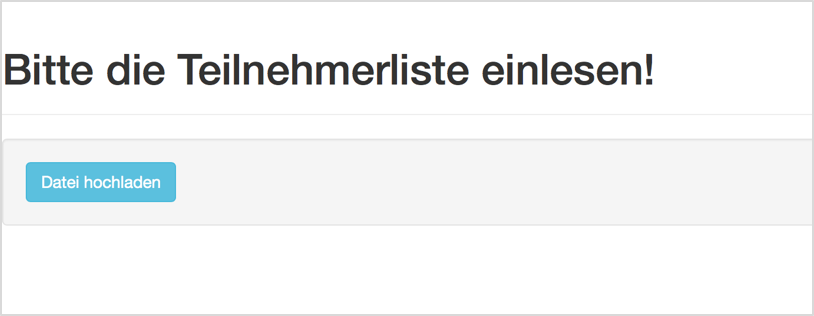
\includegraphics[width=1.0\textwidth]{FileUploader.png}
  \caption{Ausschnitt der Benutzeroberfläche des FileUploaders}
  \label{fig:Fig1}
\end{figure}
\begin{figure}[htbp]
  \centering
  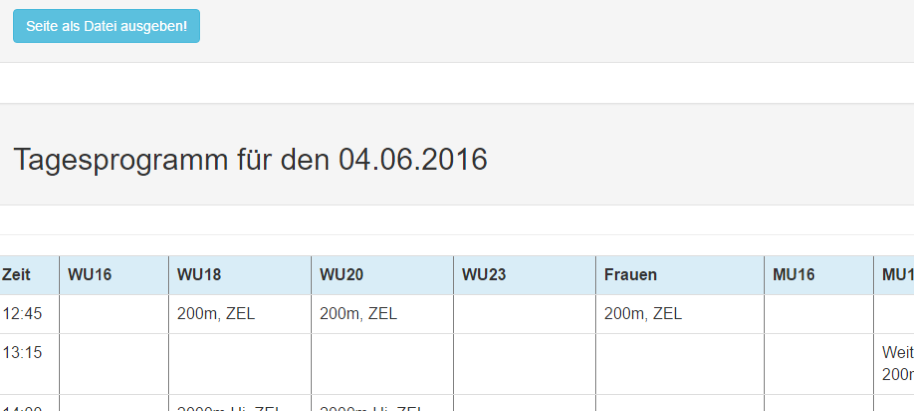
\includegraphics[width=1.0\textwidth]{Table.png}
  \caption{Ausschnitt der Benutzeroberfläche von GenerateTable}
  \label{fig:Fig1}
\end{figure}\\
Nach der Fertigstellung des Zeitplan-Generators wird dieser der Öffentlichkeit als Open Source-Software zur Verfügung gestellt. Es wird die MIT-Lizenz verwendet, da diese Lizenz viele Vorteile bietet. Ein großer Vorteil ist, dass jeder Interessierte das Tool kostenlos und in vollem Umfang nutzen kann. Des Weiteren ist es möglich, dass jeder den Code des Zeitplan-Generators nachvollziehen bzw. überprüfen kann. Bei Bedarf kann der Nutzer also auch das Tool nach seinen Vorstellungen anpassen und den Code auf Richtigkeit bzw. Qualität überprüfen. Zudem schützt die Verwendung der MIT-Lizenz die Autoren, da eine Garantie- und Rechtsverletzung ausgeschlossen werden. Die Autoren können also bei möglichen Schäden oder Ansprüchen nicht zur Verantwortung gezogen werden.\protect{\footnote{\url{https://opensource.org/licenses/MIT}, abgerufen am 13.01.17}} \\
Das herausgegebene Paket enthält die vier Web-Dokumente FileUploader, ParagraphHandler, Cleaner und GenerateTable, die die Funktionalität des Zeitplan-Generators beinhalten. Des Weiteren sind die für die Desktop-App benötigten Dateien index.html, main.js und package.json Teil des Pakets. Dies beinhaltet die verschiedenen Module von node.js, die jQuery- bzw. Bootstrap-Version und das Icon. \\
\\
Darüber hinaus wird ein README-File erstellt, das den Nutzer über die Desktop-App informiert. Das File erklärt zunächst, wo der Zeitplan-Generator eingesetzt werden kann und für wen die Nutzung interessant ist. Der Zeitplan-Generator erzeugt einen Zeitplan für Leichtathletikveranstaltungen aus einer bestimmten Ursprungsdatei. Unter dem Stichpunkt Requirements wird die benötigte Struktur und das Format der Ursprungsdatei erläutert (vgl. 2.1.2). Zudem ist das Tool kompatibel, wenn der Nutzer bisher seinen Zeitplan mit dem Tool von Seltec (www.seltec.at) erstellt hat. Möchte der Nutzer also einen Zeitplan für Leichtathletikveranstaltungen erzeugen und hat eine Ursprungsdatei dieser Form vorliegen bzw. verwendet bisher das Tool von Seltec, ist die Nutzung des Tools potenziell möglich.\\
Des Weiteren wird erklärt, wie der Zeitplan-Generator genutzt werden kann. Eine Möglichkeit ist, das Tool über die Datei index.html im Browser zu starten. Dabei wird die Verwendung der Browser Google Chrome oder Firefox empfohlen. \\
Die zweite Möglichkeit ist den Zeitplan-Generator als Desktop-App zu nutzen. Für die Nutzung der Desktop-App ist es nötig, dass der Nutzer Node.js und Electron installiert. Die jeweiligen Download-Links sind ebenfalls in dieser Beschreibung vorhanden. Für die Installation der Desktop-App wird die genaue Anleitung gegeben. In der Kommandozeile wird durch den Aufruf der jeweiligen Befehle für die Betriebssysteme im Verzeichnis der App diese selbst installiert (vgl. 2.2.6). Für eventuelle Schwierigkeiten bei der Installation werden zusätzlich einige weiterführende Links angegeben, die bei der Problemlösung helfen.\\
Weitere Bestandteile des README-Files sind die Auflistung der verwendeten Skriptsprachen, Software und Frameworks, sowie die Beschreibung des Outputs des Zeitplan-Generators. Das Tool verwendet HTML5, JavaScript, jQuery, Bootstrap, Node.js und Electron. Als Output wird eine Tabelle im HTML-Format auf dem Display ausgegeben, die der Nutzer für eine weitere Verwendung am Computer abspeichern kann.
%%%%%%%%%%%%%%%%%%%%%%%%%%%%%%%%%%%%%%%%%%%%%%%%%%%%%%%%%%%%%%%%%%%%%%%%%%%%%%
